\documentclass[]{article}
\usepackage{lmodern}
\usepackage{amssymb,amsmath}
\usepackage{ifxetex,ifluatex}
\usepackage{fixltx2e} % provides \textsubscript
\ifnum 0\ifxetex 1\fi\ifluatex 1\fi=0 % if pdftex
  \usepackage[T1]{fontenc}
  \usepackage[utf8]{inputenc}
\else % if luatex or xelatex
  \ifxetex
    \usepackage{mathspec}
  \else
    \usepackage{fontspec}
  \fi
  \defaultfontfeatures{Ligatures=TeX,Scale=MatchLowercase}
\fi
% use upquote if available, for straight quotes in verbatim environments
\IfFileExists{upquote.sty}{\usepackage{upquote}}{}
% use microtype if available
\IfFileExists{microtype.sty}{%
\usepackage{microtype}
\UseMicrotypeSet[protrusion]{basicmath} % disable protrusion for tt fonts
}{}
\usepackage[margin=1in]{geometry}
\usepackage{hyperref}
\hypersetup{unicode=true,
            pdftitle={Machine Learning, Architectural Styles and Property Values},
            pdfauthor={Thies Lindenthal* (University of Cambridge) \& Erik B. Johnson (University of Alabama)},
            pdfborder={0 0 0},
            breaklinks=true}
\urlstyle{same}  % don't use monospace font for urls
\usepackage{graphicx,grffile}
\makeatletter
\def\maxwidth{\ifdim\Gin@nat@width>\linewidth\linewidth\else\Gin@nat@width\fi}
\def\maxheight{\ifdim\Gin@nat@height>\textheight\textheight\else\Gin@nat@height\fi}
\makeatother
% Scale images if necessary, so that they will not overflow the page
% margins by default, and it is still possible to overwrite the defaults
% using explicit options in \includegraphics[width, height, ...]{}
\setkeys{Gin}{width=\maxwidth,height=\maxheight,keepaspectratio}
\IfFileExists{parskip.sty}{%
\usepackage{parskip}
}{% else
\setlength{\parindent}{0pt}
\setlength{\parskip}{6pt plus 2pt minus 1pt}
}
\setlength{\emergencystretch}{3em}  % prevent overfull lines
\providecommand{\tightlist}{%
  \setlength{\itemsep}{0pt}\setlength{\parskip}{0pt}}
\setcounter{secnumdepth}{5}
% Redefines (sub)paragraphs to behave more like sections
\ifx\paragraph\undefined\else
\let\oldparagraph\paragraph
\renewcommand{\paragraph}[1]{\oldparagraph{#1}\mbox{}}
\fi
\ifx\subparagraph\undefined\else
\let\oldsubparagraph\subparagraph
\renewcommand{\subparagraph}[1]{\oldsubparagraph{#1}\mbox{}}
\fi

%%% Use protect on footnotes to avoid problems with footnotes in titles
\let\rmarkdownfootnote\footnote%
\def\footnote{\protect\rmarkdownfootnote}

%%% Change title format to be more compact
\usepackage{titling}

% Create subtitle command for use in maketitle
\providecommand{\subtitle}[1]{
  \posttitle{
    \begin{center}\large#1\end{center}
    }
}

\setlength{\droptitle}{-2em}

  \title{Machine Learning, Architectural Styles and Property Values}
    \pretitle{\vspace{\droptitle}\centering\huge}
  \posttitle{\par}
    \author{Thies Lindenthal* (University of Cambridge) \& Erik B. Johnson
(University of Alabama)}
    \preauthor{\centering\large\emph}
  \postauthor{\par}
      \predate{\centering\large\emph}
  \postdate{\par}
    \date{14 September 2019}

\usepackage{soul}
\usepackage{color}
\sethlcolor{yellow}
\usepackage{float}
\usepackage{booktabs}
\usepackage{graphicx}
\usepackage{grffile}
\usepackage{bm}
\usepackage{amsmath}
\usepackage{setspace}
\usepackage{multirow}
\doublespacing
\usepackage[backend=bibtex, style=authoryear]{biblatex}

\begin{document}
\maketitle
\begin{abstract}
This paper first introduces an algorithm that collects pictures of
individual buildings from Google Street View. Second, it trains a deep
convolutional neural network (CNN) to classify residential buildings
into architectural styles, taking into account spatial dependencies of
these styles. Third, it investigates whether architectural styles
influence house prices. For re-sales, the architectural style is a
significant determinant of transaction prices while no such effect is
found for new buildings. Additionally, we are able to provide guidance
on how to detect and overcome some of the limitations of machine
learning methods through a large-scale comparison of predictions and
expert classifications.
\end{abstract}

\hypertarget{introduction}{%
\section{Introduction}\label{introduction}}

\let\svthefootnote\thefootnote
\let\thefootnote\relax

\footnote{{*Corresponding author: Thies Lindenthal (htl24@cam.ac.uk). Replication files are available from the author's Github repository \href{https://github.com/thies}{https://github.com/thies}. Paul E. Glade and Lukas Heckmann-Umhau are thanked for exceptional research assistance. Carolin Schmidt, Peter Brummund, Mike Langen, Colin Lizieri, Franz Fuerst, Stanimira Milcheva, D'Maris Coffman, Norm Miller, Stephen Malpezzi, John Clapp, Pavel Krivenko and participants at the ASSA/AREUEA 2019 annual meeting and seminars at UCL/Bartlett and the Homer Hoyt Institute offered excellent feedback and critique on earlier versions of this paper.}}

\addtocounter{footnote}{-1}\let\thefootnote\svthefootnote

If new developments were only pleasing to the eye, so Britain's
\emph{Building Better, Building Beautiful Commission} advising
Government, nimbyism would cease and housing supply could finally reach
the levels demanded by a growing and more affluent population (The
Economist 2018). The inaugural chair of this new commission boldly
suggested that if we built \emph{``as our Georgian and Victorian
forebears built} {[}\ldots{}{]}. \emph{All objections to new building
would slip away in the sheer relief of the public''} (Scruton 2018).
Even Prince Charles, in similar spirit, put forward ten principles for
urban growth and architecture that emphasize tradition and aesthetics
(HRH The Prince of Wales 2014). When governments and princes occupy
themselves with beauty, economists surely may take a closer look as
well. In this paper, we aim to identify the architectural styles of
residential buildings using computer vision techniques and to
empirically search for any transaction price premia associated with
these styles. If aesthetics were as strong a force in the built
environment as claimed, we should indeed find a significant effect on
property prices.

This paper assesses the value of architectural aesthetics head on by
classifying the exterior styles of residential buildings using street
level images. Recent work illustrates how street level imagery and
machine learning classification is an efficient and powerful combination
for measuring previously unobserved characteristics of the urban
environment. Naik et al. (2017) describe how neighborhood demographics
may impact the physical appearance of neighborhoods. Gebru et al. (2017)
use classified vehicle make and model information to predict income,
race, education, and voting patterns at the precinct level. Glaeser et
al. (2018) predict income in New York City. Naik, Raskar, and Hidalgo
(2016) create a neighborhood safety based Streetscore which is shown to
be highly correlated with neighborhood population density and household
income. De Nadai et al. (2016) find that greenery and street facing
windows contribute to a positive appearance of safety while Liu et al.
(2017) evaluate the quality and upkeep of the built environment along
Beijing's streets.

Glaeser, Kincaid, and Naik (2018) push the level of observation from the
block, street, or street-section level to the individual
\emph{building level}. Utilizing images of buildings' exteriors
collected from Google Street
View\footnote{\href{https://www.google.co.uk/maps}{https://www.google.co.uk/maps}},
and to a lesser degree interior images from Zillow, they find that looks
matter, at least in Boston: A one standard deviation improvement of a
building's exterior is associated with an additional USD 70,000 in home
value. Intuitively, the link between good looks and value is
bi-directional: The appearance of buildings that went through
foreclosure deteriorated significantly (Glaeser, Kincaid, and Naik
2018).

Zooming in at individual buildings significantly increases the benefits
of using mass collected street level imagery in economic research:
property characteristics previously deemed ``unobservable'' can be
directly observed in an accurate, objective, automatic and therefore
cost effective way. Deriving additional variables from unconventional
data sources like 3D airborne laser scanning (or in our case Google
Street View) is fundamental since this provides ``essential determinants
influencing real estate prices {[}which{]} are constantly missing and
are not accessible in official and mass appraiser databases'' (Helbich
et al. 2013).

In this paper we suggest a method to collect a large number of images of
individual UK buildings from Google Street View, classify the depicted
buildings using deep convolutional neural networks, combine the derived
information with sales price data and, ultimately, estimate marginal
prices for the estimated building characteristics. Our work demonstrates
that utilizing pretrained convolutional neural networks to detect
complex characteristics such as housing appearances with relatively high
accuracy comes at low computational costs and is feasible with only
modestly-sized training data. Additionally, we illustrate how machine
classifications may be sensitive to photo quality by comparing machine
classifications to those made by human experts.

\hypertarget{building-styles-and-property-values}{%
\subsection{Building styles and property
values}\label{building-styles-and-property-values}}

The aesthetics of different architectural styles make for an easy
cocktail party conversation topic -- and they may also influence market
prices. Using architectural assessments by human experts, Buitelaar and
Schilder (2017) find a sizable premium of 5\% for new buildings in the
Netherlands that refer to traditional styles and a staggering 15\%
premium for new buildings that closely follow traditional shapes, facade
composition and details. Their study carefully disentangles the
architectural style from other unobserved characteristics such as
building quality, differences in location, or year of construction.
These controls are crucial, as earlier work has established that age and
style variables tend to be highly correlated. Coulson and McMillen
(2008), for instance, suggest a non-parametric estimator and establish a
U-shaped age function and distinct price discounts for postwar and
contemporary styles (vis-à-vis more historic styles). Francke and Minne
(2017) investigate the depreciation of residential real estate in the
Netherlands and decompose land versus structure values singling out the
effect of ``physical deterioration, functional obsolescence and and
vintage effects''. They find that buildings from the 1930s carry a
strong price premium.

A large scale assessment of buildings' exteriors will allow for an
analysis of the externalities of architecture. Buildings hardly ever
stand in isolation and Ahlfeldt and Mastro (2012) investigate the
influence a building's architecture exerts on its surroundings. They
observe a positive price effect for residential buildings in the direct
proximity of iconic homes by Frank Lloyd Wright in Oak Park, Illinois. A
building's exterior does not need to be an architectural masterpiece to
co-determine the value of other houses close by. Homogeneity of building
shapes within street segments does influence property values. A
similarly shaped neighboring building is value enhancing while proximity
to a wildly different neighboring shape, everything else remaining
equal, is detrimental to property values (Lindenthal 2017a).

Unfortunately, the traditional approaches chosen by e.g. Buitelaar and
Schilder (2017) or Ahlfeldt and Mastro (2012) do not scale well. Each
observation has to be classified into architectural styles by a human
expert, which is time-consuming and costly, imposing an upper limit on
the number of observations and the level of detail captured for each
observation in any given sample. Google Street View offers a solution to
this nexus as it captures the images of almost all buildings in many
cities around the world at high level of accuracy and detail. The
challenge we address in this paper is to extract and utilize building
level information from this ubiquitous sensor, using freely available
deep learning techniques.

\hypertarget{ml-classification-of-building-styles}{%
\section{ML classification of building
styles}\label{ml-classification-of-building-styles}}

\hypertarget{image-collection}{%
\subsection{Image collection}\label{image-collection}}

The first challenge when trying to collect building images in the UK is
fundamental: How can one identify the building of interest correctly?
Simply looking up an address on Google Maps too often leads to imprecise
`street views' and not the building-level portraits needed. Fig.
\ref{fig:84Vin} presents a typical result from an address level search,
showing a broad ensemble of buildings instead of singling out the
building of interest (in this case, the partly captured terraced house
at the very left margin).

\begin{center}
  -- Insert Figure \ref{fig:84Vin} about here --
\end{center}

Previous work sourcing imagery from Google Street View has mostly
focused on neighborhood or precinct characteristics where exact spatial
assignment of objects is not required and street-level images suffice.
For major US cities, the accuracy of building image search results is
higher, which should help studies such as Glaeser, Kincaid, and Naik
(2018).

Self-evidently, the images we use for classifying architectural style
must focus on specific buildings of interest. For the UK, and many other
countries, the Google Street View API returns the coordinates of the
nearest camera snapshot for a given location but fails to provide an
accurate orientation and zoom-level of the camera needed to capture the
front of the building. To estimate the best possible view, we combine
Street View metadata queries and Ordnance Survey maps to find the
optimal camera orientation to center images on the front door of the
building of interest.

\begin{center}
  -- Insert Figure \ref{fig:fan} about here --
\end{center}

Specifically, we first look up the nearest Google Street View panorama
point (green dot in Figure \ref{fig:fan}) based on the centroid (red
dot) coordinates of a given building obtained from Ordnance Survey maps.
We then perform a viewshed analysis and identify which exterior walls
are visible from the panorama point, ignoring any wall segments where
the direct line of sight from the panorama point is obstructed by other
buildings. We can then estimate the camera bearing (green line) and zoom
factor, based on the fan of the lines of sight (in
blue).\footnote{Code necessary to replicate this analysis is available from the author's GitHub.com code repositories: \href{https://github.com/thies}{https://github.com/thies}.}

Obstructed lines of sight due to greenery, fences, garden walls or large
vehicles cannot be detected from the Ordnance Survey maps. We therefore
use a first stage image classification procedure to identify if the
building image is obstructed and we proceed the second-closest location
if the line of sight is obstructed.

By combining land registry maps with the snapshot location, we are able
to automatically build a set of building frontage images for
approximately 48,000 properties in Cambridge (UK). The Ordnance Survey
maps do not provide any use type classifications so we collect images on
all buildings that have a ground plate between 40 and 250 \(m^2\). This
method, however, could easily be adapted to photograph buildings in
locations for which high-resolution building level maps are not
available by using LIDAR based building outlines instead, which would be
in the spirit of Glaeser et al. (2018).

\hypertarget{from-pixels-to-computer-vision}{%
\subsubsection{From pixels to computer
vision}\label{from-pixels-to-computer-vision}}

We download all pictures at the highest resolution offered by Google's
Street View
API\footnote{\href{https://developers.google.com/maps/documentation/streetview/intro}{https://developers.google.com/maps/documentation/streetview/intro}}
(640x640 color pixels). We then obtain 2048-dimensional feature vectors
for each picture, using the \emph{Inception-v3} deep convolutional
neural network (Szegedy et al. 2015). \emph{Inception-v3} has been
trained for the ImageNet Large Scale Visual Recognition Challenge
(ILSVRC)\footnote{\url{http://image-net.org/challenges/LSVRC/}}, which
evaluates image classification and object detection algorithms for a
wide range of objects. The pretrained classifications would allow us to
identify pets, vehicles or people on the pictures -- assessing
architectural style, however, is beyond the canned classifiers'
capabilities.

Glaeser, Kincaid, and Naik (2018) rely on an different ILSVRC
competitor, \emph{Resnet-101} (He et al. 2016). They reduce the
extracted feature vectors to lower dimensionality (1024 to 100
dimensions) based on principal component analysis (PCA). We follow a
different strategy and double the dimensionality by including the
feature vector of the closest building in the sample, which, in most
cases, is the direct neighbor. The feature vectors of neighbors have
been collected in exactly the same way as those for other buildings in
the sample. Doubling up allows us to model spatial dependencies in
building styles, similar to spatially correlated land cover
classifications in Ghimire, Rogan, and Miller (2010).

\hypertarget{image-classification}{%
\subsection{Image classification}\label{image-classification}}

Cambridge's houses can be classified into seven broad styles:
\footnote{We are grateful to colleagues from the Architecture Department at the University of Cambridge to provide these general style descriptions.}

\begin{itemize}
\item
  \emph{Georgian} (c1714--1837) houses feature key characteristics such
  as sash windows, fan lights above doors, the use of stucco on facades,
  often wrought work grilles, railings etc.\label{def_eras}
\item
  In the \emph{Early Victorian} era (c1837--c1870s), a growing taste for
  individualized embellishment led to the development of elaborate
  features such as carved barge boards or finials. The development of
  sheet glass led to sash windows becoming more affordable, and,
  increasingly, wider.
\item
  In the \emph{Late Victorian} era (c1870s--1901), bay windows became
  more and more widespread, and increasingly substantial. Stylistic
  movements such as the Queen Anne revival style contributed richly
  ornamental details to the formal repertoire employed by designers.
  Stained glass became more popular.
\item
  \emph{Edwardian} architecture (1901-1910) tends to be less ornate than
  late Victorian architecture.
\item
  The \emph{Interwar} period (1918--1939) saw the cost of building
  construction fall, amidst a drive to provide better housing for the
  working classes. New housing types were being favored.
\item
  The \emph{Postwar} (1950-1980) styles continued on this path, with an
  embrace of high-rise as well as low rise housing. Facades vary greatly
  between brick, tiling, pebbledash and render.
\item
  The cut-off year for our \emph{Contemporary} era to begin is 1980.
  \emph{Revival} style-homes are contemporary buildings trying to
  emulate historic, mostly Victorian, architecture.
\end{itemize}

Two final-year architectural students classified a large sub-sample of
approximately 25,000 images from our data set of Cambridge
houses.\footnote{The full set of classified images are available for download at the authors' websites.}
This is a much larger sample than needed in our case. In our case, each
category requires less than 250 observations to reach saturated training
accuracy levels. We greatly exceed this number for the purpose of this
paper so that we can compare the out-of-sample convolutional neural
network predictions to the architects' classifications. This allows us
to examine the power and size of the assignment tests. In addition
having both human and machine classification for a large sample of the
data allows for robustness checks on the machine comparisons.

We create stratified training samples of 600 buildings from each
category but \emph{Georgian}, which is the least common style in
Cambridge and for which we can only sample 330 examples. This leaves a
sufficiently sized out-of-sample verification data set of 21,000 homes.

The multinomial classifier model design remains parsimonious, comprising
of:

\begin{itemize}
\item
  an input layer the size of the feature vectors, e.g.~2048 or 4096,
  respectively,
\item
  one dense layer (relu) half the size of the input layer, one
  subsequent dropout (rate 0.5) layer,
\item
  one dense layer (relu) a quarter the size of the input layer, one
  subsequent dropout (rate 0.5) layer,
\item
  and the final dense output layer with softmax activation.
\end{itemize}

All classifiers are implemented using the Keras/Tensorflow
APIs\footnote{Keras: \href{https://keras.io/}{https://keras.io/}, Tensorflow: \href{https://github.com/tensorflow/tensorflow}{https://github.com/tensorflow/tensorflow}}.
The computational burden of this rather shallow model design is modest.

For 100 randomly drawn data sets, all stratified on style, we train two
models each: The first is based on the building specific feature vectors
(2048 dimensions) only while the second also incorporates the feature
vector of the nearest neighbor (combined 4096 dimensions). In cases
where trees, fences or large vehicles obstruct the view or where the
front of a building cannot be classified with high certainty, the image
of the nearest neighbor provides a ``second opinion'' that is spatially
correlated with the observation of interest. Finally we classify all
buildings not used in training or evaluating the model (truly
out-of-sample).

When classifying a building picture, each models returns a vector of
style-scores, each between 0 to 1, that jointly sum up to 1. We select
the style with the highest score as the best estimate. By not excluding
observations where multiple scores are vying for the top rank we retain
as many observations as possible but risk a higher misclassification
rate.

Two variables are obtained from the distribution of classifications per
observation: The ensemble classifier arrives at predictions by majority
vote. In addition, a confidence measure is computed as the Herfindahl
index of classifications by ensemble member models. If, for instance, 20
models classified a building as \emph{Contemporary} but 80 others as
\emph{Revival}, the ensemble majority vote is \emph{Revival}. The
corresponding Herfindahl score is calculated as
\((20/100)^2 + (80/100)^2 = 0.68\).

We tabulate confusion matrices and evaluate the classification
performance in terms of recall, precision and \(F_1\)-scores. More
formally, the next step regresses the style classifications by
architects, captured by binomial variables \(D_{TrueVint}\), against a
vector of hedonic variables \(\mathbf{X}\), vectors of year
\(\mathbf{Y}\) and neighborhood \(\bm{Loc}\) dummy variables and the
building's \(\mathbf{Style}\), estimated both with and without spatial
dependencies. The intercept is denoted by \(\alpha\) while
\(\bm{\beta}\), \(\bm{\delta}\), \(\bm{\gamma}\) and \(\bm{\lambda}\)
are vectors of regression coefficients, and \(\epsilon\) is the error
term.

\begin{equation} \label{eq:rev}
  logit( D_{TrueVint,i} ) = \alpha + \beta\mathbf{X_i} + \delta\mathbf{Style}_i +  \gamma\mathbf{Y}_i + \lambda\mathbf{Loc}_i +  \epsilon_i
\end{equation}

The logit regressions are estimated by generalized least squares. For a
well-performing classifier, the \(\delta\) coefficients will be
statistically significant and, more importantly, differences in the
Akaike Information Criterion (AIC) allow for comparisons across the
suggested ML classifiers.

Will the resulting classifiers be biased with respect to property
values, picking up correlated but irrelevant cues such as greenery,
upkeep, or cars brands instead of building exteriors? Are, for instance,
more valuable houses more likely to be classified as the popular
\emph{Late Victorian} style while starter homes are disproportionally
more likely to be classified as e.g. \emph{Early Victorian}? We expect
that in cases in which the ensemble provided a high confidence score,
building features are clearly detectable on the pictures. For close
calls, however, where models within the ensemble cannot agree, other
factors might tilt the scale towards an incorrect class. A sizable
difference in estimated marginal prices for machine's classifications
versus the estimates for architects' classifications in the subsequent
hedonic regression (Eq. \ref{eq:hed}, below) would indicate such a bias.

\hypertarget{architectural-styles-and-property-values}{%
\section{Architectural styles and property
values}\label{architectural-styles-and-property-values}}

\hypertarget{residential-transaction-data}{%
\subsection{Residential transaction
data}\label{residential-transaction-data}}

Residential real estate transactions are public data in the UK,
collected and published by the Land Registry (Land Registry 2017). The
records include the date of transaction, price paid, street address, a
classification of the property type (flat, detached, semi-detached, or
terraced house), the estate type (freehold or leasehold) and an
indicator for newly built properties. We select transactions from
Cambridge proper which were recorded between January 1995 and October
2018, excluding any leaseholds, flats and properties classified as type
``other'', and sales with prices below £50,000 or in excess of
£2,000,000. Linking recently taken images to sales data from 24 years
assumes that houses have not changed their architectural styles -- which
seems reasonable. We are not aware of any conversions of just the
exterior of buildings. In case of full redevelopments, we exclude any
sales for a given address pre-dating the redevelopment, ensuring that a
currently taken pictures represents the house at all included
transactions. Table \ref{tab:sumstats} presents summary statistics for
the sample.

\begin{center}
  -- Insert Table \ref{tab:sumstats} about here --
\end{center}

The Ordnance Survey \emph{AddressBase} (Ordnance Survey 2017a) links
street addresses to building outlines on Ordnance Survey maps (Ordnance
Survey 2017b), which allows us to calculate the buildings floor plate
(in \(m^2\)) and to estimate the building's volume from digital
elevation models (Environment Agency 2015), as suggested by Lindenthal
(2017b). We control for the location of each building by calculating the
distance to the city center proxied by Great St.~Mary's Church, and
non-parametrically by using 69 indicator variables for each of the
smallest census tracts (\emph{Lower Super Output Areas}, LSOA)
subdividing Cambridge (Office for National Statistics 2019). LSOAs
typically have 1,000--3,000 residents and 400--1,200 households of
comparable economic and socio-demographic characteristics (Office for
National Statistics 2017).

\hypertarget{hedonic-regression-setup}{%
\subsection{Hedonic regression setup}\label{hedonic-regression-setup}}

Merging the machine's classification with sales data (Land Registry
2017) we estimate a hedonic regression equation that establishes
marginal prices for the building style (similar to Moorhouse and Smith
1994; Asabere, Hachey, and Grubaugh 1989; Vandell and Lane 1989; Fuerst,
McAllister, and Murray 2011; Plaut and Uzulena 2006), among other
characteristics: \begin{equation} \label{eq:hed}
  ln(Price_i) = \alpha + \beta\mathbf{X_i} + \delta\mathbf{Style}_i + \eta\mathbf{StyleNeigh}_i + \iota\mathbf{Style\cdot StyleNeigh}_i  +\gamma\mathbf{Y}_i + \lambda\mathbf{Loc}_i +  \epsilon_i
\end{equation}

Here, the natural logarithm of sales prices is explained by a linear
combination of hedonic attributes described in vector \(\mathbf{X}\),
vectors of year \(\mathbf{Y}\) and neighborhood \(\bm{Loc}\) dummy
variables and the building's estimated \(\mathbf{Style}\) and the
prevailing styles of other buildings in the direct proximity
\((\mathbf{StyleNeigh})\). \(\mathbf{Style\cdot StyleNeigh}\) is a
vector of interaction terms for the building's and the neighborhood's
dominant style. The intercept is denoted by \(\alpha\) while
\(\bm{\beta}\), \(\bm{\delta}\), \(\bm{\eta}\), \(\bm{\iota}\),
\(\bm{\gamma}\) and \(\bm{\lambda}\) are vectors of regression
coefficients. \(\epsilon\) is the IID error term. Heteroscedastic robust
standard errors will be reported.

Are buildings with different appearances imperfect substitutes catering
to multiple groups of households with distinct style or vintage
preferences? Buitelaar and Schilder (2017) indicate that any premium for
an architectural style must stem from either differences in construction
prices (which they do not find in their Dutch sample) or from supply
constraints, as new construction potentially does not capture the demand
for traditional styles. For Cambridge, new supply will inevitably be of
either contemporary or revival style as historic vintages (and their
styles), by definition, are not supplied any more. Estimating Eq.
\ref{eq:hed} for a subset of newly constructed buildings will show
whether construction prices or supply constraints for new homes built
according to different architectural styles persist -- if too few
vernacular buildings were built, prices should reflect such a shortage.
Singling out new buildings crucially controls for the otherwise
unobserved age of buildings, which is tightly intertwined with its
aesthetics.

\hypertarget{results}{%
\section{Results}\label{results}}

Almost 16,000 of the 25,000 buildings for which we have an architect's
classification could be matched to the 23,768 sales transactions that
have been recorded for Cambridge between 1995 and 2018. The remaining
9,000 houses have not been sold since 1995 - but the information on
their architectural style is still valuable for our measures of
neighborhood styles. Thus, we observe both the machine's and the
architects' classification for the majority of buildings in the data
set.

\begin{center}
  -- Insert Table \ref{tab:confmat} about here --
\end{center}

The agreement between classifications by the machine and by the
architects is reassuringly strong. When relying on feature vectors of
the buildings and their closest neighbors, 67 to 84 percent of true
classifications are matched with correctly estimated labels (Table
\ref{tab:confmat}, Panel A). The recall rates are especially high for
older styles: For \emph{Georgians}, it is 79 percent, \emph{Early
Victorian} 81 percent, \emph{Late Victorian/Edwardian} 78 percent,
\emph{Interwar} 84 percent, respectively. For more recent \emph{Postwar}
buildings, the rate drops to 71 percent, for \emph{Contemporary} to 72
percent and for \emph{Revival} to 67 percent.

A visual inspection of classifications is additionally reassuring.
Figure \ref{fig:vint_examples} displays the pictures which carry the
highest out-of-sample scores for each style The model is clearly able to
differentiate based on small cues, even when only parts of the facade
are captured on the picture.

The Herfindahl scores for classifications vary substantially across
styles, as classified by the architects (Table \ref{tab:herftab}),
indicating that the models within the ensemble, for instance, agree more
often on a building being \emph{Georgian} than finding consensus for
other styles. For \emph{Contemporary} or \emph{Revival} styles,
individual classifications differ most. All off-diagonal elements in the
lower panel of Table \ref{tab:herftab} are negative, suggesting that, in
general, the Herfindahl index is a good predictor of misclassified
images.

A closer inspection of the misclassified images sheds some light on the
limits of automatically collected street level imagery. What do
misclassified images have in common? Off-the-shelf object detection
algorithms can identify broadly defined objects such as trees, vehicles,
houses, doors, or windows without any additional training. Using an
Inception/Resnet object detection model trained on Open
Images\footnote{In this case, "faster rcnn inception resnet v2 atrous oidv2", available from \url{https://github.com/tensorflow/models/blob/master/research/object_detection/g3doc/detection_model_zoo.md}},
we calculate the share of the image area taken up by cars or trees as a
measure of view obstruction. The more image area is showing buildings
and, importantly, windows the more meaningful input an automatic
classifier can draw from, resulting in better classifications. In
addition, images not taken at an optimal angle or zoom factor are
detected by calculating the distance between the bounding box for the
largest building detected on the image and the center of the image: For
well-centered images, this offset will be small.

Table \ref{tab:imgqualsumstats} presents the mean values for the image
quality variables. Table \ref{tab:diffimgchar}, Panel A, compares the
mean values for views obstructed by trees or vehicles for correctly (on
diagonal) and incorrectly classified images. In most cases, the
off-diagonal values are positive, showing that more obstacles in the
view of sight correlate with a higher likelihood of misclassifications.
Similarly, if more of the image area shows a house (Panel B),
misclassifications are reduced (negative differences). This effect is
stronger for windows, which appear to give valuable cues about a house's
style (Panel C). Finally, houses that are not in the center of the
building tend to be misclassified more frequently (positive differences
in Panel D). In sum, bad quality images lead to misclassifications.

\begin{center}
  -- Insert Table \ref{tab:herftab}, Table \ref{tab:imgqualsumstats} and Table \ref{tab:diffimgchar} about here --
\end{center}

The number of misclassifications decreases decidedly when considering
observations with high ensemble confidence only: The majority vote based
on the most confident two-thirds of machine classifications only are
more in line with the architects' classifications, as higher recall,
precision and \(F_1\)-scores in Table \ref{tab:confmat}, Panel B, show.
The improvement is most evident in the precision rates. For the
relatively rare categories of \emph{Georgian} and \emph{Revival} about
the same number of buildings classified as \emph{Georgian/Revival} in
Panel A actually belong to a different style, according to the human
experts. The precision shoots up from 0.50 to 0.70 for \emph{Georgian}
and from 0.52 to 0.82 for \emph{Revival} when excluding the not so
confident lower third of predictions in Panel B.

The majority of misclassification is concentrated in temporally adjacent
eras: 10 percent of \emph{Late Victorian/Edwardian} buildings are
labelled as \emph{Early Victorian} or 18 percent of \emph{Postwar}
buildings are erroneously regarded as stemming from the \emph{Interwar}
period. Hardly ever is a contemporary building mistaken for a historic
home.

\begin{center}
  -- Insert Figure \ref{fig:vint_examples} about here --
\end{center}

Overall, the spatial softmax classification incorporating the nearest
neighbor's feature vector outperforms the base classifier: pairwise
differences of the \(F_1\)-scores from the spatial and the base
classifier are clearly positive (Fig. \ref{fig:boxplot}). AIC values for
28 binomial models based on Eq. \ref{eq:rev} decrease as hedonic
characteristics, location and time dummies are augmented by the base and
spatial ML predictor (Table \ref{tab:aic}). For all building styles, the
AIC are lowest for the spatial ML predictor. In sum, the spatial
classifier performs better for UK style data than a classifier based on
single buildings only.

\begin{center}
  -- Insert Table \ref{tab:aic} and Figure \ref{fig:boxplot} about here --
\end{center}

\hypertarget{hedonic-regression-estimates}{%
\subsection{Hedonic regression
estimates}\label{hedonic-regression-estimates}}

Successively, the estimated coefficients from 8 different versions of
the hedonic regression specified in Eq. (\ref{eq:hed}) are reported in
Tables \ref{tab:hedreg} and \ref{tab:hedregint}. For all models, the
hedonic control variables show the expected signs: Negative coefficients
for the relative distance to the city center, discounts for terraced
homes and semi-detached homes relative to detached houses, positive
elasticities for building floor plate and building volumes and a price
premium for new buildings compared to second-hand homes. Year and
neighborhood dummies control for time effects and local amenities but
their coefficients are not reported due to space constraints. The
combination of location dummies and the distance to the city center
measure controls for proximity to the city center \emph{within} each
neighborhood.

\begin{center}
  -- Insert Table \ref{tab:hedreg} about here --
\end{center}

The first column in Table \ref{tab:hedreg} presents the estimated
regression coefficients for the architects' classifications. The base
style \emph{Contemporary} is more expensive than almost all other
styles, which show negative coefficients that are significantly
different from 0. A clear pecking order appears: \emph{Georgian} and
\emph{Revival} buildings demand the highest premium \((+0.04)\),
followed by \emph{Late Victorian/Edwardian} \((+0.01)\),
\emph{Contemporary} (base), \emph{Early Victorian} \((-0.13)\),
\emph{Interwar} \((-0.15)\) and \emph{Postwar} \((-0.22)\).

The sample images classified by architects is not necessarily
representative of the overall population so we re-estimate the model
using machine classifications for \emph{all} buildings for which we were
able to extract usable pictures from Google Street View. Overall, the
style coefficients become more positive relative to the base, implying
that our automatic classification is biased and tends to classify
unattractive buildings to the \emph{Contemporary} style. Reversely, more
attractive buildings are disproportionally often misclassified as
\emph{Late Vic./Edw.}, pushing up the corresponding coefficient to
\(0.11\). This bias vanishes in the third model, which uses only
confidently estimated machine styles (Column 3).

Models 4--6 follow the same logic as 1--3 but are estimated for
\emph{new} buildings only. Basically this contrasts houses which might
\emph{look} different from the street, having either contemporary or
revival facades, but which are all modern homes at their core.
Differences in e.g.~materials, floor plans, green space and gardens are
minimal. For newly built homes, no effect of \emph{Revival} architecture
on price can be found for high confidence ML estimates, neither for
classifications by machines nor by architects. After controlling for
location, building characteristics and quality, buyers show no
willingness to pay a premium for \emph{Revival} architecture (Columns 4
and 6).

Introducing a variable capturing the most prominent style of buildings
on the same street and within 100 m (\(\mathbf{VintNeigh}\)) does not
change the pecking order of building styles much (Table
\ref{tab:hedreg}, Column 7). Neighboring styles are compared to the base
case of a \emph{Contemporary} house in a \emph{Contemporary} street. The
negative coefficients on dissimilar neighboring styles support a finding
by Lindenthal (2017b) that shows that a harmonious match of a building's
shape with its direct environment leads to a price premium -- or a
discount in case of shape mismatches. In relative terms, \emph{Postwar}
buildings are the least popular neighbors. The difference between
\emph{Revival} and \emph{Contemporary} neighbors is not statistically
significant. We fail to find evidence in favor of positive externalities
from revival architecture. Everything else equal, buildings within
ensembles of \emph{Contemporary} generally do not achieve higher
transaction prices than buildings in more historic areas (as Table
\ref{tab:comb} will confirm later).

Table \ref{tab:hedregint} presents the \(\iota\) interaction
coefficients (Eq. \ref{eq:hed}) for style-neighboring style combinations
with sufficient numbers of observations (see Table \ref{tab:vintneigh}).
The last row suggests that a general claim that \emph{Revival} neighbors
exert positive externalities and increase property values relative to
\emph{Contemporary} surroundings cannot be confirmed empirically. Again,
we find no statistically significant difference.

\begin{center}
  -- Insert  Table \ref{tab:vintneigh}, Table \ref{tab:hedregint} and Table \ref{tab:comb} about here --
\end{center}

In Table \ref{tab:comb}, the combined effect of building styles on
property values is calculated by adding up the direct, neighborhood and
interaction effects (Tables \ref{tab:hedreg} and \ref{tab:hedregint}).
When filling in lots in historical neighborhoods, however, a premium for
\emph{Revival} facades over modern designs can be observed (differences
in last two columns of Table \ref{tab:comb}). For large scale new
construction, however, \emph{Revival} buildings surrounded by other
historicizing buildings do not sell for more than \emph{Contemporary}
buildings in a more modern setting.

\hypertarget{conclusion}{%
\section{Conclusion}\label{conclusion}}

The contributions of this paper are threefold: First, it introduces an
algorithm that collects pictures of \emph{individual} buildings from
Google Street View. Earlier work has not achieved this level of detail
and was, at least in the UK, limited to street sections only. A
large-scale application of automatic classification of individual
buildings' characteristics using Google Street View has potential not
only in the UK. The image collection and classification method can
easily be ported to other study areas which have existing Street View
data and either LIDAR based building outlines or high resolution
satellite images. In a follow-up project, we are working on an improved
classification workflow in which a customized object detection model is
able to recognize specific building outlines without the need for
additional maps or other data.

Second, we developed a new database of 25,000 building pictures that
have been classified by architecture experts into relevant architectural
styles. We subsequently trained a neural network classifier to
automatically classify all residential buildings of a mid-sized English
city into architectural styles. The suggested classifier is trained on
feature vectors of buildings and their nearest neighbors to exploit
spatial correlation in observed classifications.

The large ground truth data set allows for a comparison of human expert
versus machine classifications. Poor image quality, for instance
obstructed views or the lack of informative features such as windows, is
correlated with misclassifications. Importantly, for cases in which the
ML classifiers are relatively indecisive between classes, visual cues
that are correlated with the exterior's style but not part of a
building's architecture (for instance trees or cars) bias the estimates.
Fore these less certain cases, more valuable homes are systematically
more likely to be classified as e.g. \emph{Late Victorian/Edw.} and less
likely to be considered \emph{Contemporary}. A follow up study could
investigate which elements in the building pictures lead to the
misclassifications (Ribeiro, Singh, and Guestrin 2016). Given the danger
of systematic biases, one should remain wary of ML estimates derived
from data sets sizable enough to train models -- but too small to
investigate any biases.

Third, we test whether revival or vernacular architecture leads to price
premia over contemporary architecture. We do not find evidence for a
preference of residents for specific architecture after controlling for
quality and location of buildings. This applies to both direct price
effects but also indirect effects of a buildings appearance on the value
of neighboring homes. Further work will extend the spatial scope of the
study area to the UK in general and to other countries.

\newpage
\clearpage

\hypertarget{tables-and-figures}{%
\section{Tables and Figures}\label{tables-and-figures}}

\begin{figure}[hbt]
  \caption{`Street View', not `Building View' -- Identification of buildings remains a challenge in the UK}
  \centering
  \vspace{0.25cm}
    \includegraphics[width=0.8\textwidth]{figures/84VineryRD.png}
  \label{fig:84Vin}
\begin{minipage}{0.8\textwidth}
\footnotesize 
\vspace{0.25cm}
\emph{Notes:} For the UK, the Google Street View API returns the coordinates of the nearest camera snapshot for a given location but fails to provide an accurate orientation and zoom-level of the camera needed to capture the front of the building exactly. In this typical example, the building of interest is only partially shown at the very left margin of this result.  \emph{Image source}: Google Street View. 
\end{minipage}
\end{figure}

\begin{figure}[hbt]
  \caption{Image Collection on Google Street View: Camera Direction and Zoom}
  \centering
    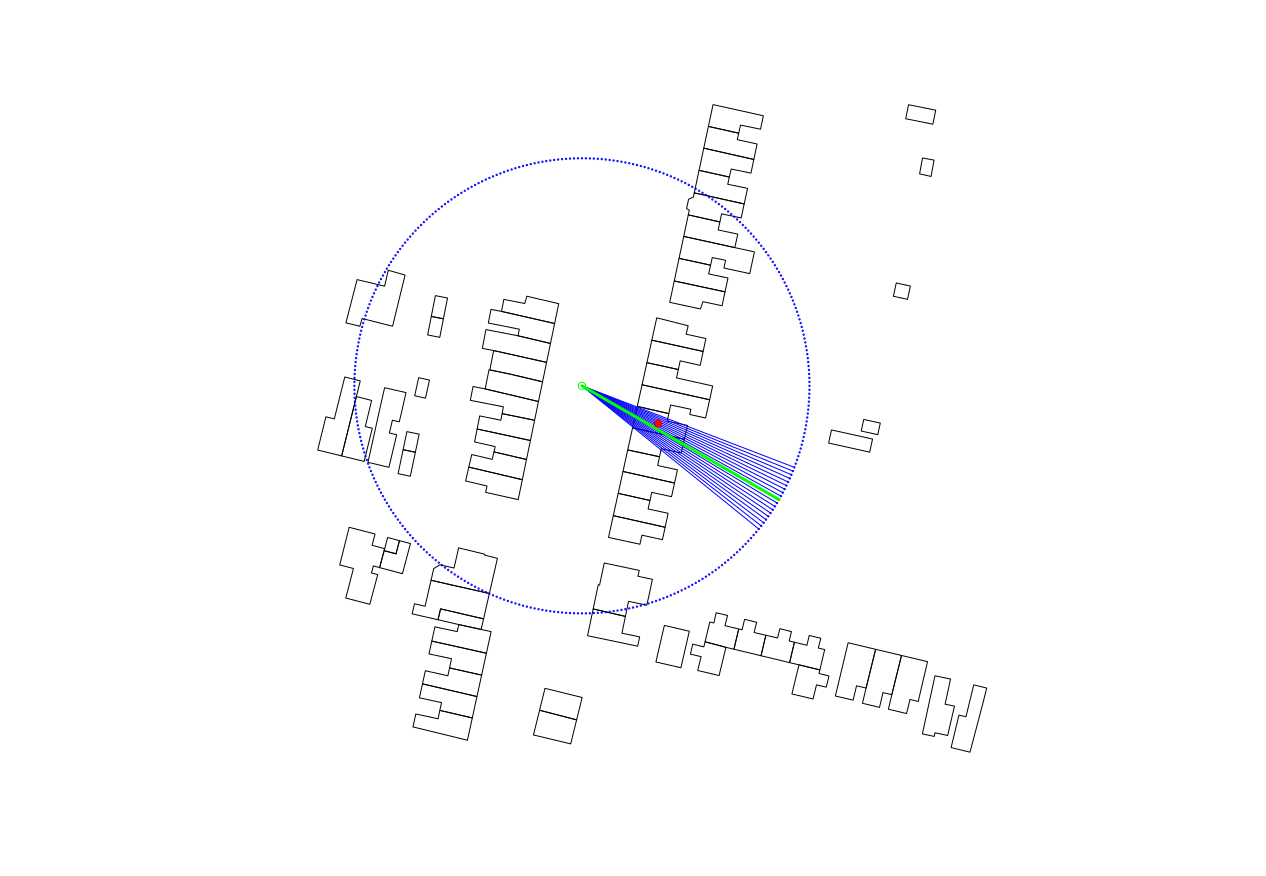
\includegraphics[width=0.8\textwidth]{figures/fan.png}
  \label{fig:fan}
\begin{minipage}{0.8\textwidth}
\vspace{0.25cm}
\footnotesize \emph{Notes:} We first look up the nearest Google Street View panorama point (green dot) based on the centroid (red dot) coordinates of a given building obtained from Ordnance Survey maps. A viewshed analysis identifies which exterior walls are visible from the panorama point, ignoring any wall segments where the direct line of sight from the panorama point is obstructed by other buildings. The camera bearing (green line) and zoom factor are based on the angle of the most outer lines of sight (blue lines).
\end{minipage}
\end{figure}

\begin{table}[!htbp] \centering 
  \caption{Summary statistics residential property transactions} 
  \label{tab:sumstats} 
\begin{tabular}{@{\extracolsep{5pt}}lccccccc} 
\toprule
Statistic & \multicolumn{1}{c}{N} & \multicolumn{1}{c}{Mean} & \multicolumn{1}{c}{St. Dev.} & \multicolumn{1}{c}{Min} & \multicolumn{1}{c}{Pctl(25)} & \multicolumn{1}{c}{Pctl(75)} & \multicolumn{1}{c}{Max} \\ 
\midrule
Price & 23,768 & 253,646.20 & 170,987.20 & 10,000 & 127,000 & 326,374.8 & 1,000,000 \\ 
Year & 23,768 & 2,004.89 & 6.59 & 1,995 & 1,999 & 2,010 & 2,018 \\ 
ln(volume) & 23,768 & 286.00 & 188.14 & 0.00 & 215.50 & 370.89 & 1,926.45 \\ 
ln(area) & 23,768 & 63.25 & 28.44 & 4.94 & 45.74 & 72.46 & 1,058.70 \\ 
ln(dist. city center) & 23,768 & 2,477.63 & 1,007.55 & 112.78 & 1,652.39 & 3,166.05 & 5,023.62 \\ 
New & 23,768 & 0.04 & 0.20 & 0 & 0 & 0 & 1 \\ 
Type: detached & 23,768 & 0.13 & 0.34 & 0 & 0 & 0 & 1 \\ 
Type: semi-detached & 23,768 & 0.35 & 0.48 & 0 & 0 & 1 & 1 \\ 
Type: terraced & 23,768 & 0.52 & 0.50 & 0 & 0 & 1 & 1 \\ 
Georgian & 23,768 & 0.03 & 0.16 & 0 & 0 & 0 & 1 \\ 
Early Vic. & 23,768 & 0.15 & 0.36 & 0 & 0 & 0 & 1 \\ 
Late Vic./Edw. & 23,768 & 0.21 & 0.40 & 0 & 0 & 0 & 1 \\ 
Interwar & 23,768 & 0.32 & 0.47 & 0 & 0 & 1 & 1 \\ 
Postwar & 23,768 & 0.23 & 0.42 & 0 & 0 & 0 & 1 \\ 
Contemporary & 23,768 & 0.03 & 0.17 & 0 & 0 & 0 & 1 \\ 
Revival & 23,768 & 0.04 & 0.20 & 0 & 0 & 0 & 1 \\ 
Neigh: Georgian & 23,768 & 0.02 & 0.12 & 0 & 0 & 0 & 1 \\ 
Neigh: Early Vic. & 23,768 & 0.14 & 0.35 & 0 & 0 & 0 & 1 \\ 
Neigh: Late V./Edw. & 23,768 & 0.22 & 0.41 & 0 & 0 & 0 & 1 \\ 
Neigh: Interwar & 23,768 & 0.32 & 0.47 & 0 & 0 & 1 & 1 \\ 
Neigh: Postwar & 23,768 & 0.25 & 0.43 & 0 & 0 & 1 & 1 \\ 
Neigh: Contemporary & 23,768 & 0.02 & 0.15 & 0 & 0 & 0 & 1 \\ 
Neigh: Revival & 23,768 & 0.03 & 0.18 & 0 & 0 & 0 & 1 \\ 
\bottomrule
\end{tabular} 
\begin{minipage}{\textwidth}
\vspace{0.25cm}
\singlespacing
\footnotesize \emph{Notes:} Summary statistics for sample of 23,768 residential real estate transactions for the city of Cambridge (UK) between 1995 and 2018 where buildings could be matched with Google Street View images. The buildings floor plate (in $m^2$) is based on OS maps and the buildings' volumes are estimated from digital elevation models, as suggested by @Lindenthal2017a. We control for the location of each building by calculating the distance to the city center proxied by Great St. Mary's Church, and non-parametrically by using 69 location dummies (based on LSOA). Building styles based on machine classifications.
\end{minipage}
\end{table}

\begin{table}[!htb]
	\caption{Confusion matrix for classification based on images of property and its nearest neighbor}
	\label{tab:confmat}
	\centering
\begingroup\footnotesize
	\emph{}
\begin{tabular}{lrrrrrrr}
	& \multicolumn{7}{c}{\rule{0pt}{4ex}    \emph{Panel A: Model based on individual building and nearest neighbor} \rule{0pt}{4ex}    }\\
	\toprule
	\emph{Machine} & \multicolumn{7}{c}{\emph{Architects}} \\
	\cmidrule(lr){2-8}
	& Georgian & Early Vic. & Late V./Edw. & Interwar & Postwar & Cont. & Revival \\
  \cmidrule(lr){1-1}
\cmidrule(lr){2-8}
	Georgian & 284 & 109 & 77 & 38 & 14 & 23 & 22 \\
	  Early Vic. & 50 & 1755 & 427 & 86 & 86 & 56 & 34 \\
	  Late V./Edw. & 10 & 172 & 3260 & 213 & 56 & 21 & 29 \\
	  Interwar & 10 & 46 & 254 & 5884 & 997 & 56 & 54 \\
	  Postwar & 1 & 17 & 48 & 514 & 3914 & 74 & 40 \\
	  Cont. & 3 & 50 & 63 & 101 & 333 & 855 & 69 \\
	  Revival & 3 & 29 & 45 & 139 & 145 & 98 & 501 \\
		\cmidrule(lr){1-1}
\cmidrule(lr){2-8}
	  Georgian & 79\% & 5\% & 2\% & 1\% & 0\% & 2\% & 3\% \\
	  Early Vic. & 14\% & 81\% & 10\% & 1\% & 2\% & 5\% & 5\% \\
	  Late V./Edw. & 3\% & 8\% & 78\% & 3\% & 1\% & 2\% & 4\% \\
	  Interwar & 3\% & 2\% & 6\% & 84\% & 18\% & 5\% & 7\% \\
	  Postwar & 0\% & 1\% & 1\% & 7\% & 71\% & 6\% & 5\% \\
	  Cont. & 1\% & 2\% & 2\% & 1\% & 6\% & 72\% & 9\% \\
	  Revival & 1\% & 1\% & 1\% & 2\% & 3\% & 8\% & 67\% \\
		\cmidrule(lr){1-1}
\cmidrule(lr){2-8}
	  Recall & 0.79 & 0.81 & 0.78 & 0.84 & 0.71 & 0.72 & 0.67 \\
	  Precision & 0.50 & 0.70 & 0.87 & 0.81 & 0.85 & 0.58 & 0.52 \\
	  $F_1$-score & 0.61 & 0.75 & 0.82 & 0.82 & 0.77 & 0.64 & 0.59 \\

		\cmidrule(lr){1-1} \cmidrule(lr){2-8}
		& \multicolumn{7}{c}{ \emph{ Panel B: Model based on individual building and nearest neighbor, high confidence only} \rule{0pt}{4ex}    }\\
		\cmidrule(lr){1-1} \cmidrule(lr){2-8}

Georgian & 122 & 31 & 9 & 4 & 2 & 1 & 5 \\
Early Vic. & 30 & 1,926 & 324 & 19 & 40 & 15 & 7 \\
  Late V./Edw. & 0 & 105 & 2,941 & 68 & 19 & 0 & 9 \\
 Interwar & 6 & 6 & 81 & 3,230 & 369 & 10 & 14 \\
 Postwar & 0 & 3 & 5 & 96 & 1,831 & 9 & 6 \\
 Cont. & 0 & 8 & 7 & 4 & 33 & 236 & 18 \\
 Revival & 3 & 2 & 0 & 14 & 10 & 4 & 154 \\
 \cmidrule(lr){1-1}
\cmidrule(lr){2-8}
 Georgian & 76\% & 2\% & 0\% & 0\% & 0\% & 0\% & 2\% \\
 Early Vic. & 19\% & 93\% & 10\% & 1\% & 2\% & 6\% & 3\% \\
  Late V./Edw. & 0\% & 5\% & 87\% & 2\% & 1\% & 0\% & 4\% \\
 Interwar & 4\% & 0\% & 2\% & 94\% & 16\% & 4\% & 7\% \\
 Postwar & 0\% & 0\% & 0\% & 3\% & 80\% & 3\% & 3\% \\
 Cont. & 0\% & 0\% & 0\% & 0\% & 1\% & 86\% & 9\% \\
Revival & 2\% & 0\% & 0\% & 0\% & 0\% & 2\% & 72\% \\
\cmidrule(lr){1-1}
\cmidrule(lr){2-8}
Recall & 0.76 & 0.93 & 0.87 & 0.94 & 0.79 & 0.86 & 0.72 \\
 Precision & 0.70 & 0.82 & 0.94 & 0.87 & 0.94 & 0.77 & 0.82 \\
$F_1$-score & 0.73 & 0.87 & 0.90 & 0.90 & 0.86 & 0.81 & 0.77 \\

\cmidrule(lr){1-1} \cmidrule(lr){2-8}
& \multicolumn{7}{c}{ \emph{Panel C: Model based on individual buildings only} \rule{0pt}{4ex}    }\\
\cmidrule(lr){1-1} \cmidrule(lr){2-8}

	Georgian & 267 & 121 & 110 & 46 & 33 & 36 & 17 \\
	  Early.Vic. & 50 & 1673 & 438 & 112 & 107 & 63 & 52 \\
	  Late V./Edw. & 19 & 183 & 3099 & 272 & 86 & 33 & 44 \\
	  Interwar & 12 & 71 & 335 & 5786 & 1419 & 84 & 82 \\
	  Postwar & 2 & 24 & 56 & 462 & 3364 & 75 & 38 \\
	  Cont. & 5 & 63 & 82 & 141 & 366 & 778 & 79 \\
	  Revival & 6 & 43 & 54 & 156 & 170 & 114 & 437 \\
	\cmidrule(lr){1-1}
\cmidrule(lr){2-8}
	  Georgian & 74\% & 6\% & 3\% & 1\% & 1\% & 3\% & 2\% \\
	  Early.Vic. & 14\% & 77\% & 10\% & 2\% & 2\% & 5\% & 7\% \\
	  Late V./Edw. & 5\% & 8\% & 74\% & 4\% & 2\% & 3\% & 6\% \\
	  Interwar & 3\% & 3\% & 8\% & 83\% & 26\% & 7\% & 11\% \\
	  Postwar & 1\% & 1\% & 1\% & 7\% & 61\% & 6\% & 5\% \\
	  Cont. & 1\% & 3\% & 2\% & 2\% & 7\% & 66\% & 11\% \\
	  Revival & 2\% & 2\% & 1\% & 2\% & 3\% & 10\% & 58\% \\
		\cmidrule(lr){1-1}
\cmidrule(lr){2-8}
	  Recall & 0.74 & 0.77 & 0.74 & 0.83 & 0.61 & 0.66 & 0.58 \\
	  Precision & 0.42 & 0.67 & 0.83 & 0.74 & 0.84 & 0.51 & 0.45 \\
	  $F_1$-score & 0.54 & 0.72 & 0.78 & 0.78 & 0.70 & 0.58 & 0.51 \\
	 \bottomrule
\end{tabular}

\begin{minipage}{\textwidth}
\footnotesize
\vspace{0.25cm}
	\emph{Notes:} Cross-tabulation of out-of-sample predictions by the machine versus the architects' classification.
	\emph{Recall} is the share of buildings from an architects' category being predicted correctly (diagonal in mid panel) and \emph{Precision} is the share of buildings predicted to belong to a category that are indeed from that category.
	$F_1$-scores are the harmonious mean of Precision and Recall: \emph{ $F_1$-score = 2 Recall * Precision / (Recall + Precision).}
\end{minipage}


\endgroup
\end{table}


\begin{table}[!htb] 
\caption{Prediction certainty: Herfindahl index from ensemble model} 
\label{tab:herftab} 
\footnotesize
\begin{tabular}{lccccccc}
\toprule 
  & \multicolumn{7}{c}{\emph{Architects}} \\ 
  \cmidrule(lr){2-8} 
& Georgian &  Early Vic. & Late V. /Edw. & Interwar & Postwar & Cont. & Revival \\  

Mean Herf. & 0.88 &  0.80 & 0.79 & 0.77 & 0.68 &  0.70 &  0.70 \\  
 \midrule 
\emph{Machine} & \multicolumn{7}{c}{\emph{Difference from correct classifications (diagonal), t-stats in parenthesis}} \\
\cmidrule(lr){2-8} 
Georgian & -- & -0.21 (-9.87) & -0.28 (-13.11) & -0.33 (-9.95) & -0.27 (-6.30) & -0.25 (-7.97) & -0.25 (-7.54) \\
 Early Vic. & -0.22 (-6.28) &  -- & -0.19 (-19.20) & -0.31 (-13.70) & -0.21 (-10.05) & -0.21 (-7.53) & -0.15 (-3.84) \\
 Late V./Edw. & -0.36 (-5.89) & -0.24 (-18.03) &  -- & -0.26 (-21.88) & -0.23 (-9.08) & -0.24 (-4.96) & -0.16 (-4.33) \\
 Interwar & -0.12 (-1.55) & -0.32 (-12.77) & -0.24 (-19.87) &  -- & -0.13 (-22.67) & -0.25 (-12.58) & -0.16 (-6.49) \\
 Postwar & -0.51 (-33.71) & -0.30 (-6.24) & -0.36 (-13.13) & -0.26 (-34.82) & -- & -0.22 (-10.34) & -0.24 (-7.70) \\
 Cont. & -0.44 (-3.31) & -0.37 (-17.78) & -0.38 (-17.63) & -0.39 (-25.39) & -0.18 (-15.67) & -- & -0.19 (-7.71) \\
 Revival & -0.09 (-0.42) & -0.40 (-20.64) & -0.41 (-22.54) & -0.31 (-19.71) & -0.28 (-24.06) & -0.22 (-12.40) &  -- \\
\bottomrule 
\end{tabular}
\begin{minipage}{\textwidth}
\vspace{0.25cm}
\footnotesize \emph{Notes:} For each ensemble classification $i$, we derive the Herfindahl scores as the sum of the squared share of votes from individual models for each of the 7 styles $s$ received, calculated as: $Herf_i=\sum_{s=1}^{s=7} (votes_s/votes_{all})^2$. A high score indicates high levels of consensus within the ensemble. The Herf. scores tend to be lower at off-diagonal cells, indicating lower consensus for misclassifications.
\end{minipage}
\end{table}

\begin{table}[ht] 
\centering 
 \caption{Mean Values for image quality variables, by style}
 
\label{tab:imgqualsumstats}
\begin{tabular}{lcccc} 
\toprule 
Architects' classifications & Share Blocked & House Area & Window Area & Image Offset \\ 
\midrule
 Georgian & 0.07 & 0.81 & 0.15 & 0.07 \\ 
 Early Vic. & 0.06 & 0.86 & 0.16 & 0.05 \\ 
 Late V./Edw. & 0.11 & 0.84 & 0.17 & 0.08 \\ 
 Interwar & 0.19 & 0.70 & 0.11 & 0.12 \\ 
 Postwar & 0.16 & 0.64 & 0.07 & 0.11 \\ 
 Cont. & 0.09 & 0.72 & 0.11 & 0.09 \\ 
 Revival & 0.10 & 0.78 & 0.11 & 0.09 \\ 
 \bottomrule
\end{tabular}
\begin{minipage}{0.9\textwidth}
\vspace{0.25cm}
\footnotesize \emph{Notes:} Using an Inception/Resnet object detection model trained on Open Images, basic object on the images are detected and the share of the image area taken up by cars, trees, buildings and windows are calculated. Images taken not taken at an optimal angle or zoom factor are detected by calculating the offset between the bounding box for the largest detected building and the center of the image.
\end{minipage}
\end{table}

\begin{table}[!htb] 
\caption{Difference in photo characteristics by correctly and incorrectly classified images} 
\label{tab:diffimgchar} 
\centering 
\begingroup\scriptsize 
\begin{tabular}{lrrrrrrr}

\toprule 

\emph{Machine} & \multicolumn{7}{c}{\emph{Architects}} \\ 
  \cmidrule(lr){2-8} 
& Georgian & Early Vic. & Late V./Edw. & Interwar & Postwar & Cont. & Revival \\  

 \cmidrule(lr){2-8} 
 & \multicolumn{7}{c}{\emph{ Panel A: Total share of house blocked by vehicles or trees}}\\ 
\cmidrule(lr){1-1} \cmidrule(lr){2-8} 

Georgian &  -- &  0 (0.16) & -0.03 (-1.37) & -0.07 (-2.16) & -0.06 (-0.91) & -0.02 (-0.86) &  0.02 (0.39) \\  
  Early Vic. & -0.04 (-2.80) &  -- & -0.04 (-7.42) & -0.11 (-8.26) & -0.09 (-5.45) & -0.03 (-1.97) &  0.01 (0.47) \\  
  Late V./Edw. &  0.03 (0.91) &  0.03 (2.55) &  -- &  0.01 (0.40) &  0.01 (0.57) &  0.01 (0.17) &  0.08 (1.89) \\  
  Interwar &  0.17 (2.24) &  0.11 (3.71) &  0.09 (5.73) &  -- &  0.03 (4.16) &  0.18 (4.42) &  0.07 (2.40) \\  
  Postwar &  0.13 (0.96) &  0.03 (1.44) &  0.11 (2.88) & -0.01 (-1.20) &  -- &  0.09 (3.39) &  0.04 (1.09) \\  
  Cont. &  0.16 (0.77) & -0.02 (-1.91) &  0.03 (1.14) & -0.03 (-0.92) & -0.04 (-3.06) &  -- & -0.03 (-1.32) \\  
  Revival &  0.18 (0.74) &  0.03 (0.92) &  0.01 (0.26) & -0.05 (-3.03) & -0.06 (-4.90) &  0.04 (2.02) &  -- \\  

\cmidrule(lr){1-1} \cmidrule(lr){2-8} 
 & \multicolumn{7}{c}{\emph{ Panel B: Share of house area}}\\ 
\cmidrule(lr){1-1} \cmidrule(lr){2-8} 

  Georgian &  -- & -0.11 (-3.43) & -0.10 (-2.67) &  0.09 (1.94) &  0.10 (0.96) &  0.11 (1.29) & -0.02 (-0.31) \\  
  Early Vic. &  0.05 (1.30) &  -- &  0.03 (1.75) &  0.07 (2.45) &  0.18 (5.01) &  0.12 (2.19) &  0.05 (1.03) \\  
  Late V./Edw. & -0.09 (-2.08) & -0.07 (-3.10) &  -- &  0.02 (1.07) &  0.08 (2.23) & -0.08 (-1.29) &  0.04 (0.71) \\  
  Interwar &  0.08 (0.55) & -0.16 (-3.68) & -0.14 (-6.48) &  -- &  0.03 (2.92) & -0.04 (-1.03) & -0.09 (-2.65) \\  
  Postwar & -0.33 (-1.98) & -0.24 (-3.82) & -0.18 (-3.25) & -0.05 (-4.60) &  -- & -0.12 (-2.78) & -0.16 (-4.57) \\  
  Cont. & -0.21 (-1.58) & -0.16 (-2.99) & -0.15 (-3.45) & -0.02 (-0.55) &  0.01 (0.23) &  -- & -0.06 (-1.43) \\  
  Revival & -0.03 (-0.15) & -0.04 (-0.69) & -0.11 (-2.70) &  0.06 (2.51) &  0.08 (3.30) &  0.05 (1.30) &  -- \\  

\cmidrule(lr){1-1} \cmidrule(lr){2-8} 
 & \multicolumn{7}{c}{\emph{ Panel C: Share of window area}}\\ 
\cmidrule(lr){1-1} \cmidrule(lr){2-8} 

 Georgian &  -- & -0.06 (-6.02) & -0.02 (-1.10) & -0.02 (-1.92) &  0.03 (1.26) & -0.03 (-1.28) & -0.01 (-0.42) \\  
  Early Vic. & -0.01 (-0.60) &  -- & -0.01 (-1.51) &  0.03 (2.72) &  0.04 (5.30) &  0.01 (0.70) &  0.02 (1.83) \\  
  Late V./Edw. &  0 (0.09) & -0.02 (-2.67) &  -- &  0.04 (4.85) &  0.02 (1.81) &  0.02 (0.98) &  0.02 (1.59) \\  
  Interwar & -0.03 (-0.92) & -0.09 (-10) & -0.08 (-13.20) &  -- &  0.01 (2.98) & -0.03 (-2.41) & -0.03 (-3.48) \\  
  Postwar & -0.07 (-4.42) & -0.09 (-5.80) & -0.08 (-4.50) & -0.02 (-4.95) &  -- & -0.05 (-4.42) & -0.05 (-5.63) \\  
  Cont. & -0.07 (-2.04) & -0.08 (-6.97) & -0.05 (-3.73) & -0.01 (-1.46) &  0.01 (2.50) &  -- & -0.02 (-2.58) \\  
  Revival & -0.02 (-0.18) & -0.06 (-4.39) & -0.03 (-1.71) &  0.01 (1.04) &  0.02 (2.50) & -0.02 (-2.33) &  -- \\    

\cmidrule(lr){1-1} \cmidrule(lr){2-8} 
 & \multicolumn{7}{c}{\emph{ Panel D: Image offset}}\\ 
\cmidrule(lr){1-1} \cmidrule(lr){2-8} 

 Georgian &  -- &  0.04 (5.44) &  0.02 (2.61) & -0.02 (-1.71) & -0.03 (-1.33) &  0.01 (1) &  0.01 (0.55) \\  
  Early Vic. &  0.01 (0.64) &  -- & -0.02 (-6.59) & -0.03 (-3.82) & -0.04 (-4.98) & -0.01 (-0.93) & -0.03 (-2.78) \\  
  Late V./Edw. &  0.04 (1.96) &  0.03 (4.68) &  -- & -0.01 (-1.25) & -0.02 (-2.14) &  0.01 (0.46) &  0 (0.25) \\  
  Interwar &  0.03 (1.16) &  0.06 (6.28) &  0.05 (9.75) &  -- &  0.01 (2.35) &  0 (0.06) &  0.03 (3.19) \\  
  Postwar &  0.04 (1.07) &  0.06 (3.31) &  0.04 (3.37) &  0 (1.11) &  -- &  0.02 (1.95) &  0.06 (4.20) \\  
  Cont. &  0.08 (2.11) &  0.05 (3.87) &  0.04 (3.40) & -0.01 (-1.32) & -0.02 (-4.26) &  -- &  0 (0.20) \\  
  Revival &  0 (0.02) &  0.03 (2.06) &  0.01 (1) & -0.01 (-1.85) & -0.01 (-1.02) &  0.02 (2.22) &  -- \\  
\bottomrule 
 
\end{tabular} 
 \begin{minipage}{\textwidth} 
\footnotesize 
\vspace{0.25cm}
\emph{Notes:} Cross-tabulation of photo characteristics by machine and architects' classifications. Off-diagonal elements ($Machine_{j}-Architects_{i}$) describe the difference in measure intensity between correctly and incorrectly classified photos for a given classification by architects. For example, cell \{Early Vic., Georgian\} compares the mean characteristic value for the set of photos which are actually Georgian but misclassified as Early Vic. to the set of correctly classified Georgian photos. The numbers in italic represent the mean characteristic value for each set of correctly classified photos. T-stats are in parenthesis.
\end{minipage} 
\endgroup 
\end{table}

\begin{figure}[htb!]
\caption{Examples of machine-based style classifications}
\begin{tabular}{lllllll}
  \hline
\emph{Georg.} & \emph{Early Vic.} & \emph{Late V./Edw.} & \emph{Interwar} & \emph{Postwar} & \emph{Contemp.} & \emph{Revival} \\ 
  \hline
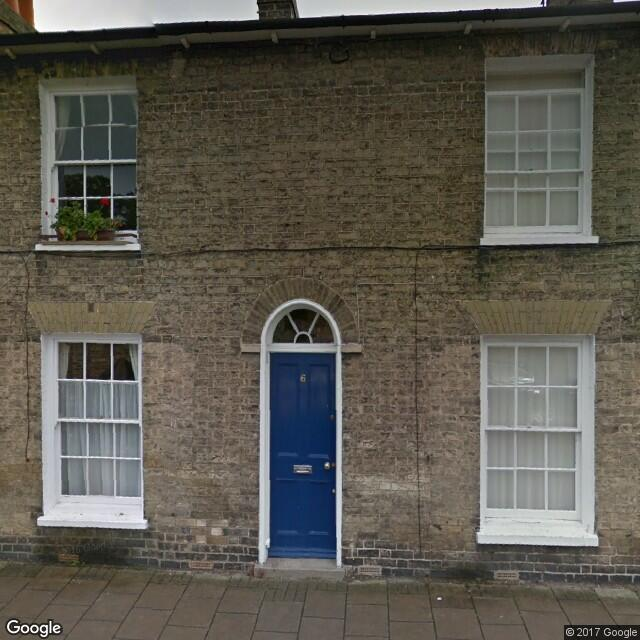
\includegraphics[width=45px]{/home/thies/db/Cambridge/data/images/cambridge/0001000010058205_KqBBtZS8ecncUe8oqjErqQ.jpg} & 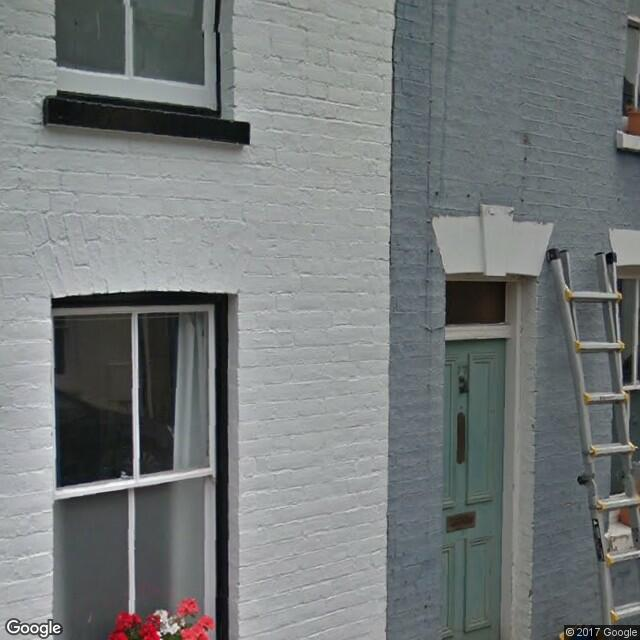
\includegraphics[width=45px]{/home/thies/db/Cambridge/data/images/cambridge/0001000010102767_u_7T3iAyG9xNgeN_ETY7aQ.jpg} & 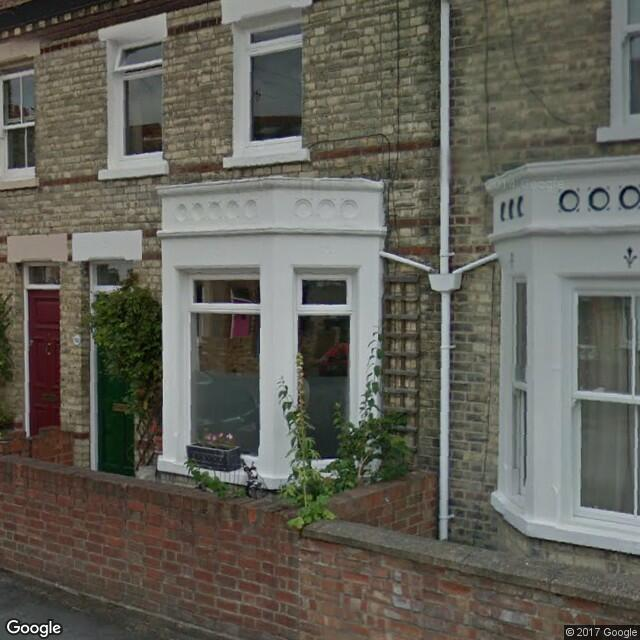
\includegraphics[width=45px]{/home/thies/db/Cambridge/data/images/cambridge/0001000010141478_FT9houQ2x66NPnNEGxTkvA.jpg} & 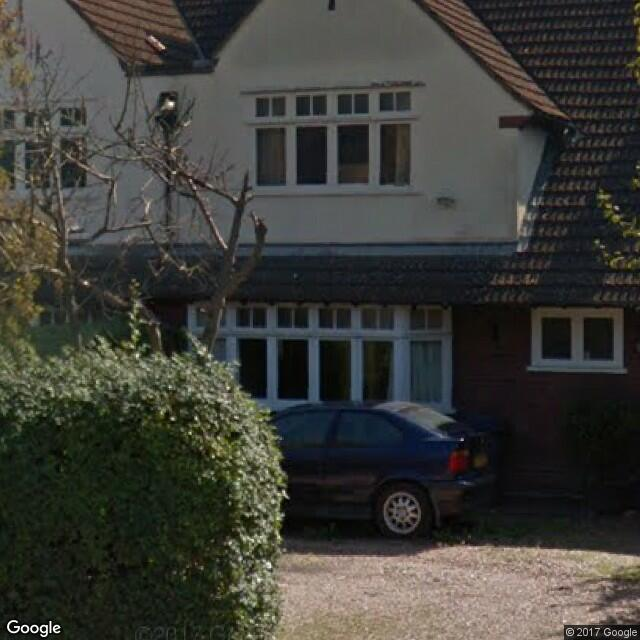
\includegraphics[width=45px]{/home/thies/db/Cambridge/data/images/cambridge/0001000010065714_pzExlR026vDKdQaJiLkdkw.jpg} & 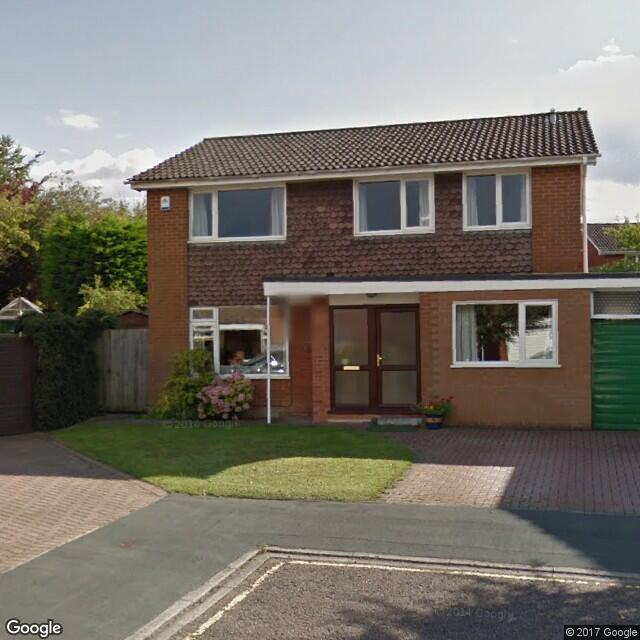
\includegraphics[width=45px]{/home/thies/db/Cambridge/data/images/cambridge/0001000010137600_qYxYCsLRPpOfCyv8IjfnlA.jpg} & 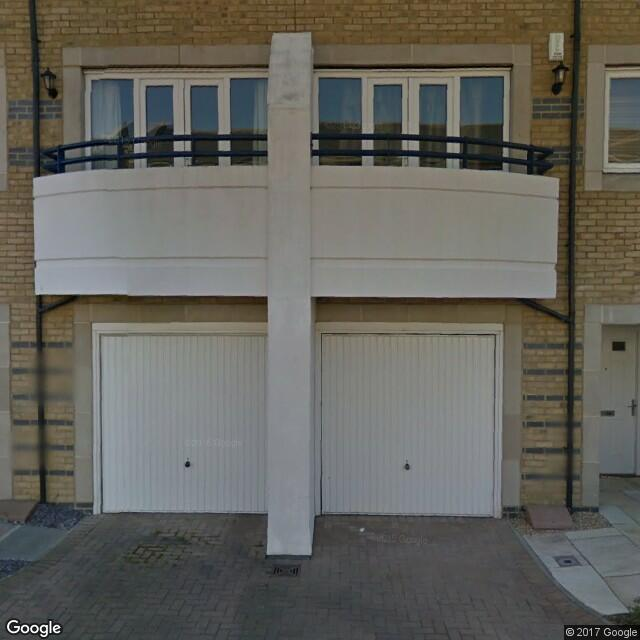
\includegraphics[width=45px]{/home/thies/db/Cambridge/data/images/cambridge/1000002057677225_srJnz_31ujVFzn-xh_DYfw.jpg} & 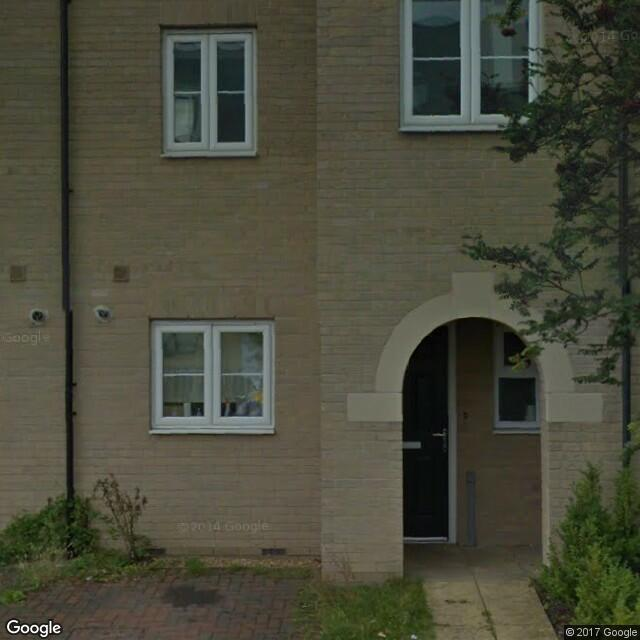
\includegraphics[width=45px]{/home/thies/db/Cambridge/data/images/cambridge/1000002500413689_VylY6Sy3vLvjqbtHeryMdQ.jpg} \\ 
  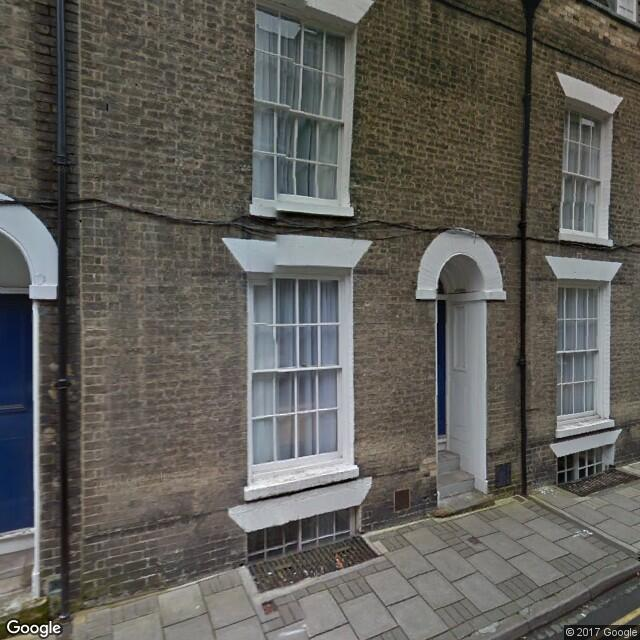
\includegraphics[width=45px]{/home/thies/db/Cambridge/data/images/cambridge/0001000010056385_XQsTJ2p5Te54CScFmblMHA.jpg} & 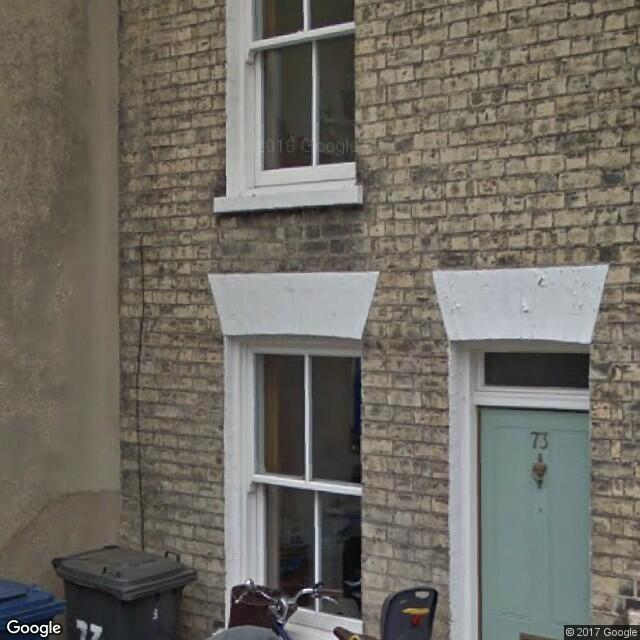
\includegraphics[width=45px]{/home/thies/db/Cambridge/data/images/cambridge/0001000010102769_c_e4WlmafqN2JXQ2ZhYEkw.jpg} & 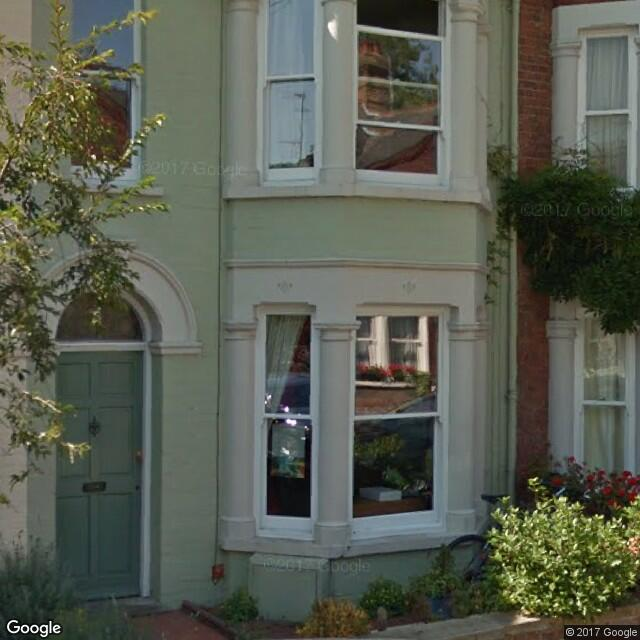
\includegraphics[width=45px]{/home/thies/db/Cambridge/data/images/cambridge/0001000010017237_yWs7fxQ0r8Ecx_ajaYc-rg.jpg} & 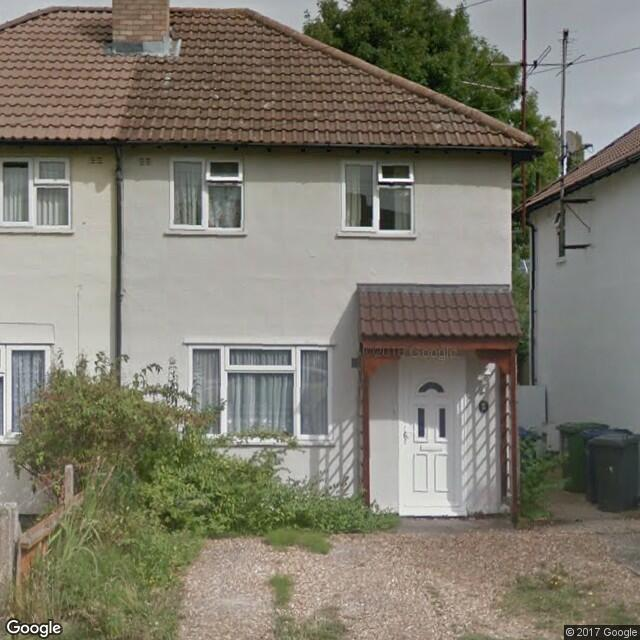
\includegraphics[width=45px]{/home/thies/db/Cambridge/data/images/cambridge/0001000010141115_xG0eSas79cN59fH4xvm5Yw.jpg} & 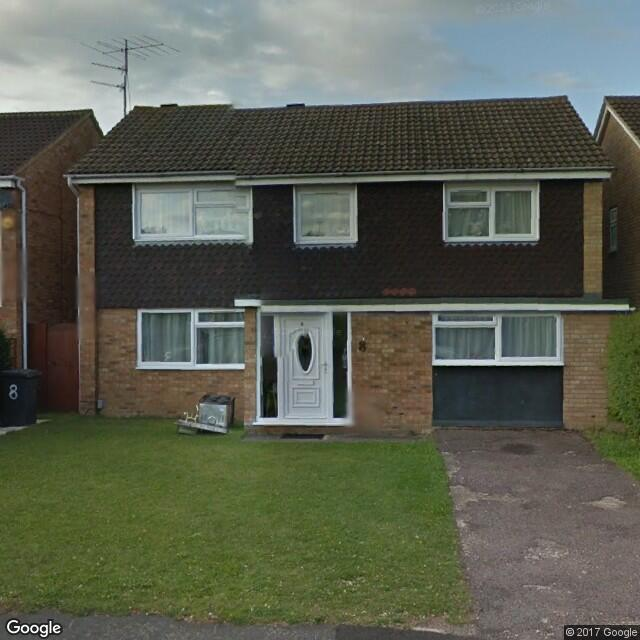
\includegraphics[width=45px]{/home/thies/db/Cambridge/data/images/cambridge/0001000010023665_B2Is2WMV8SGjf7Tg9tLS7w.jpg} & 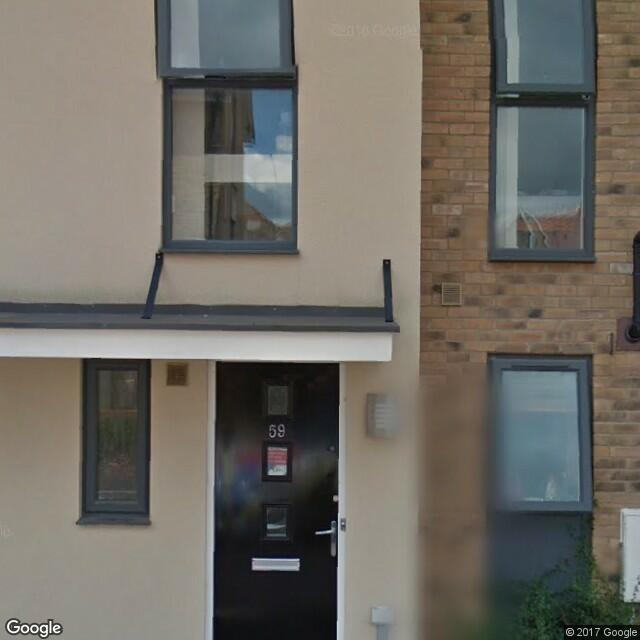
\includegraphics[width=45px]{/home/thies/db/Cambridge/data/images/cambridge/1000002500748070_DkW5iwQYtGox02-tF2i9rQ.jpg} & 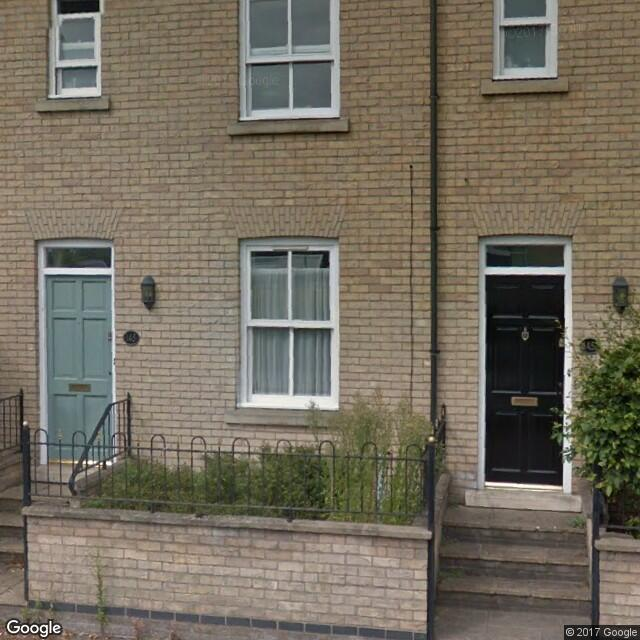
\includegraphics[width=45px]{/home/thies/db/Cambridge/data/images/cambridge/0001000010176986_bNOie2HS7GPQxPOtoevEHw.jpg} \\ 
  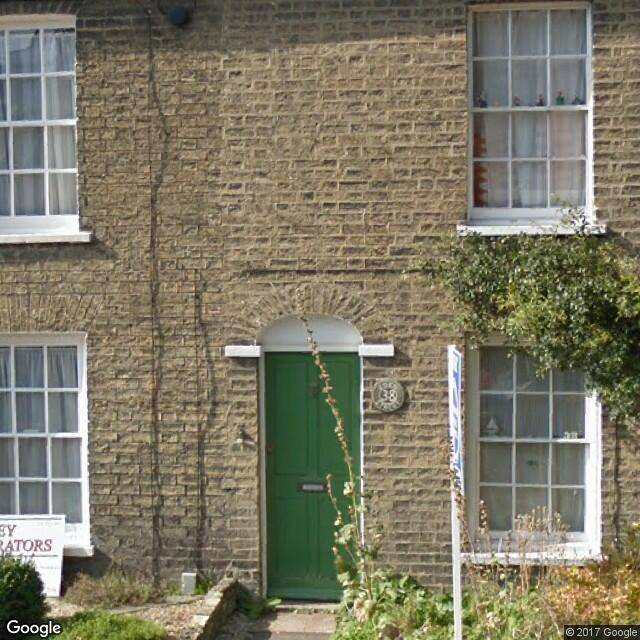
\includegraphics[width=45px]{/home/thies/db/Cambridge/data/images/cambridge/0001000010058145_xBAz4f8lI2MTivvvWv6wyQ.jpg} & 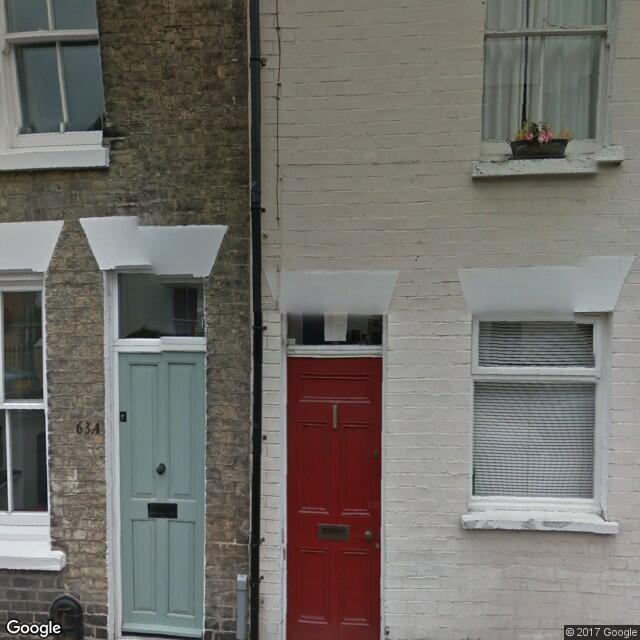
\includegraphics[width=45px]{/home/thies/db/Cambridge/data/images/cambridge/0001000010103488_Y1L2niOkEGB1IKe4tsl1yw.jpg} & 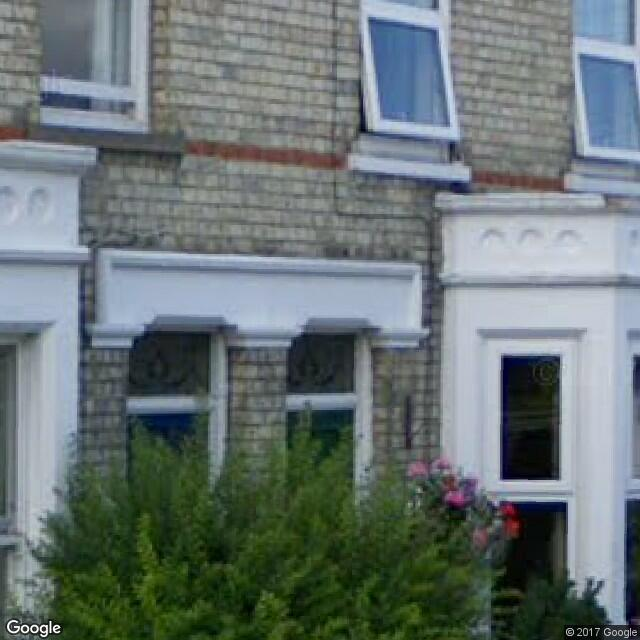
\includegraphics[width=45px]{/home/thies/db/Cambridge/data/images/cambridge/0001000010021367_JF-P4lOQQouZ6lHtM4J3oA.jpg} & 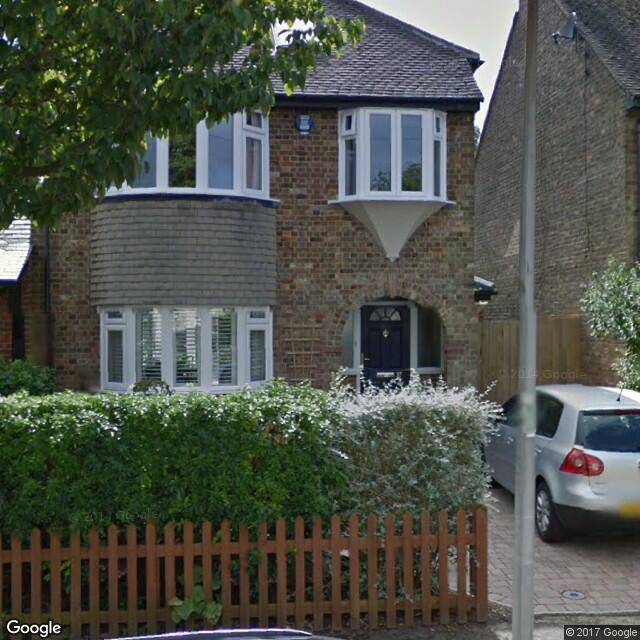
\includegraphics[width=45px]{/home/thies/db/Cambridge/data/images/cambridge/0001000010065349_HDvoqsiHXGx4xc62JSUNJA.jpg} & 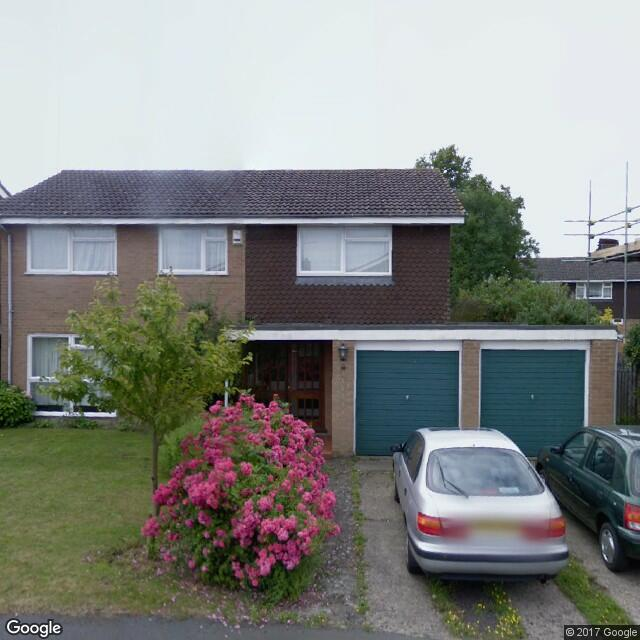
\includegraphics[width=45px]{/home/thies/db/Cambridge/data/images/cambridge/0001000009993819_748OTBKSFyJZU2DP7TbboQ.jpg} & 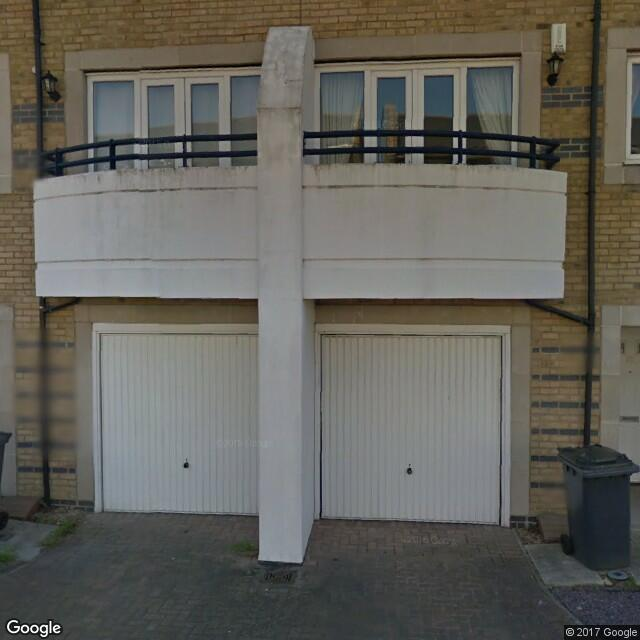
\includegraphics[width=45px]{/home/thies/db/Cambridge/data/images/cambridge/1000002057677000_8l6ywNIej2136uZeb3qKqA.jpg} & 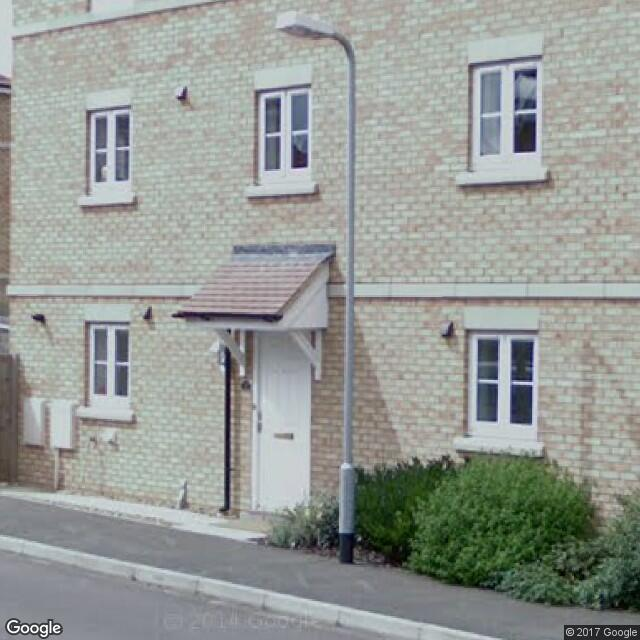
\includegraphics[width=45px]{/home/thies/db/Cambridge/data/images/cambridge/1000002500088807_4vu-eMLHmhX3JmHNwyulmQ.jpg} \\ 
  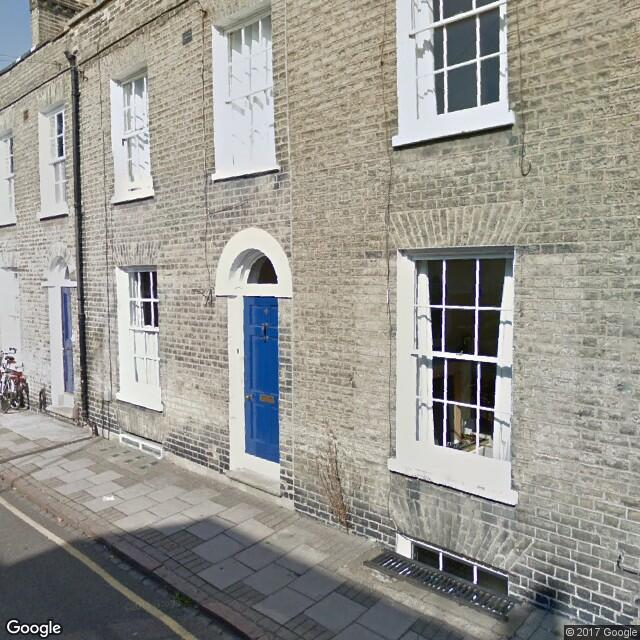
\includegraphics[width=45px]{/home/thies/db/Cambridge/data/images/cambridge/0001000010059206__nUymOPxCgpQugahoE7EPw.jpg} & 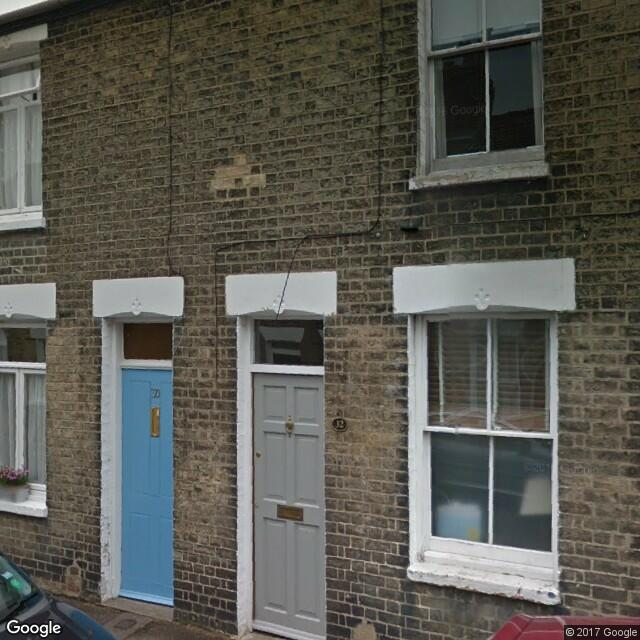
\includegraphics[width=45px]{/home/thies/db/Cambridge/data/images/cambridge/0001000010103870_ywN_BuvuLW6kbLLP0QgJMA.jpg} & 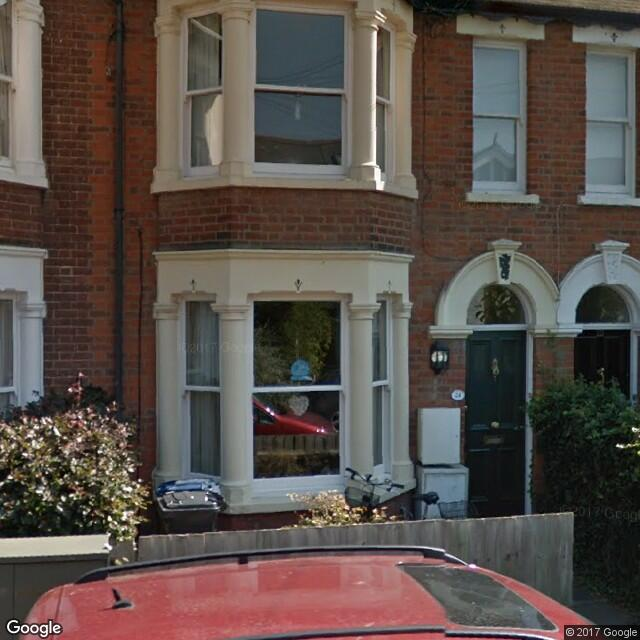
\includegraphics[width=45px]{/home/thies/db/Cambridge/data/images/cambridge/0001000010017412_aOsldmaOT-MAce6q6qkmTQ.jpg} & 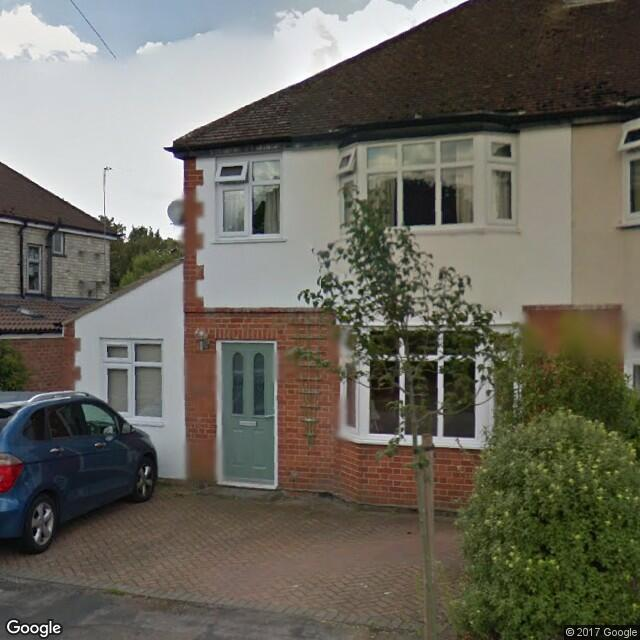
\includegraphics[width=45px]{/home/thies/db/Cambridge/data/images/cambridge/0001000010107971_veilqmDOA-AfCuz4tWyg7g.jpg} & 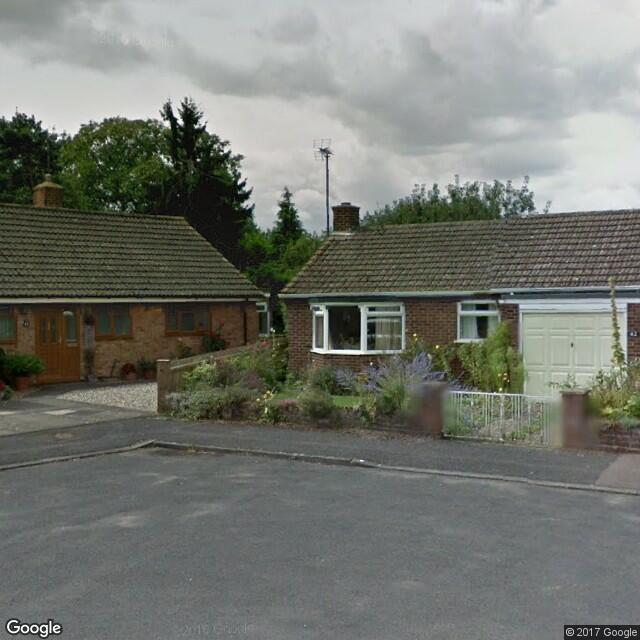
\includegraphics[width=45px]{/home/thies/db/Cambridge/data/images/cambridge/0001000010025542_8rvXwCYBTCQu0eVM9nhN9Q.jpg} & 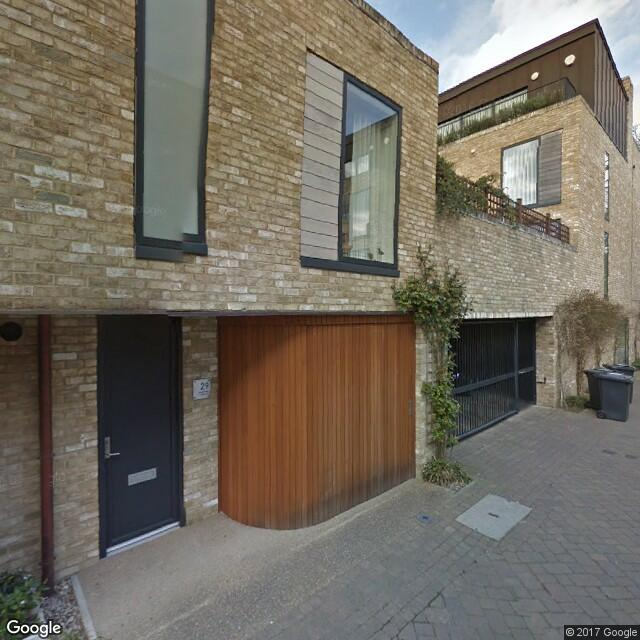
\includegraphics[width=45px]{/home/thies/db/Cambridge/data/images/cambridge/1000002500555322_FffLx_XVBUOvZgiXRdSAnA.jpg} & 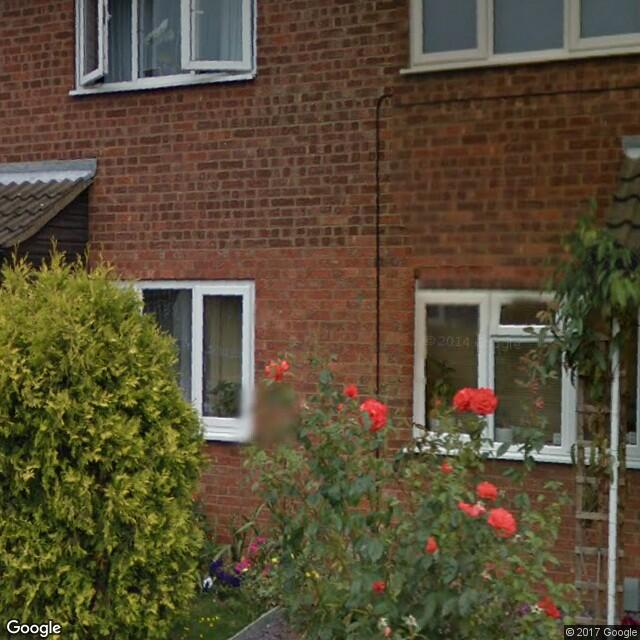
\includegraphics[width=45px]{/home/thies/db/Cambridge/data/images/cambridge/0001000010066754_dJmIRHcgebzrGzDR_Cahaw.jpg} \\ 
  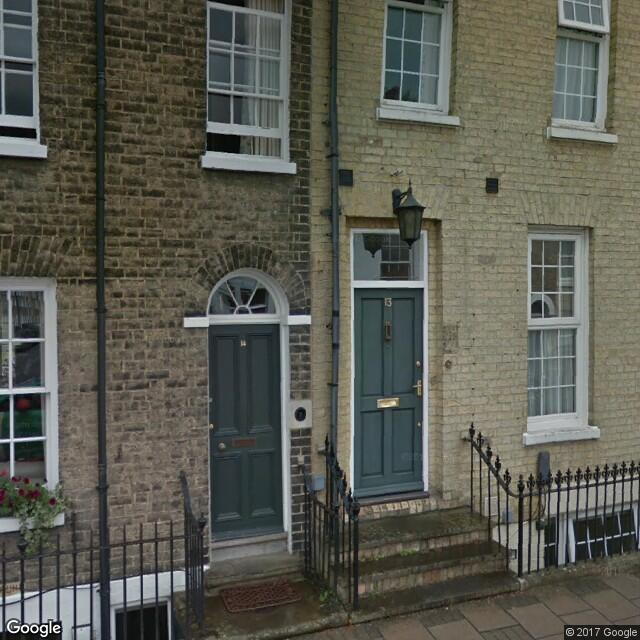
\includegraphics[width=45px]{/home/thies/db/Cambridge/data/images/cambridge/0001000010060140_8_DVq9QCmlMezNuDHGixwg.jpg} & 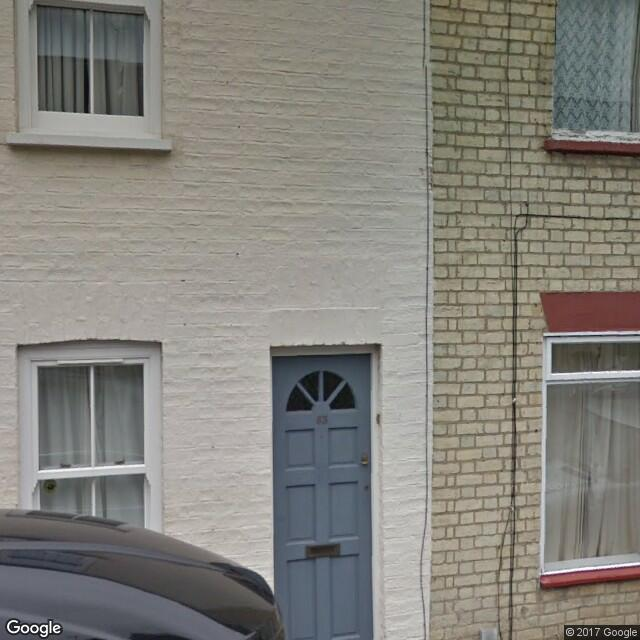
\includegraphics[width=45px]{/home/thies/db/Cambridge/data/images/cambridge/0001000010103819_mF6OqQrRTOlAoGdaraQsTQ.jpg} & 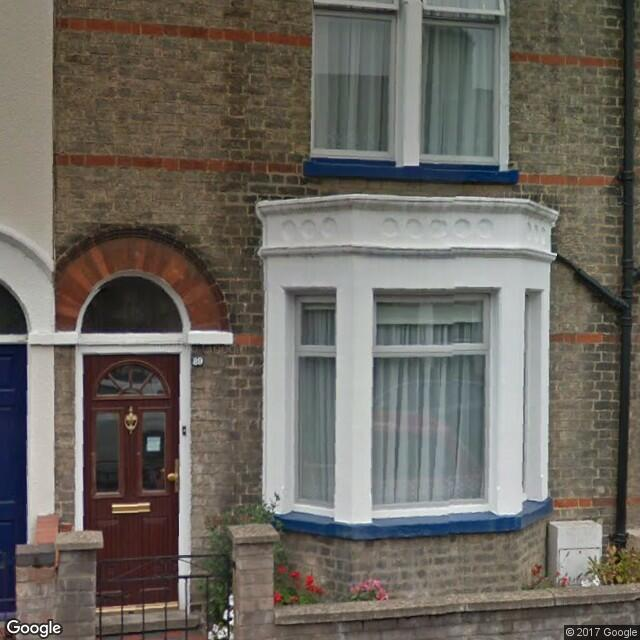
\includegraphics[width=45px]{/home/thies/db/Cambridge/data/images/cambridge/0001000010097999_xTD3YceIrtPJZwPz5d0G6Q.jpg} & 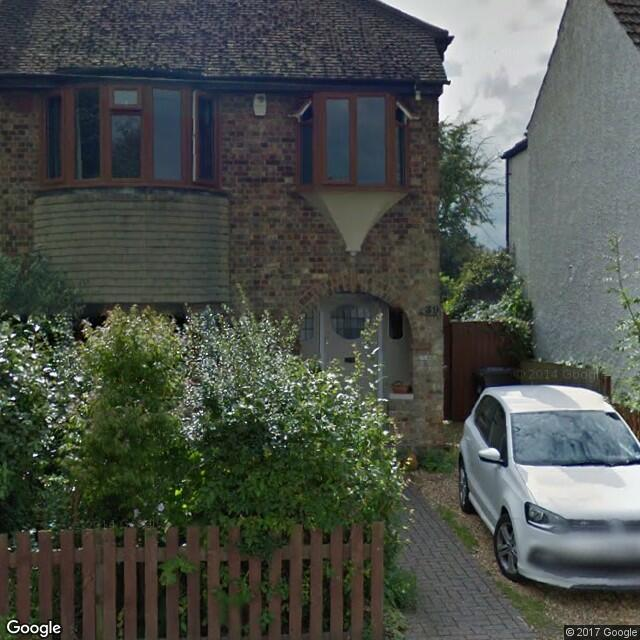
\includegraphics[width=45px]{/home/thies/db/Cambridge/data/images/cambridge/0001000010065347_pouLRqJd7pkk41jryvYQ4A.jpg} & 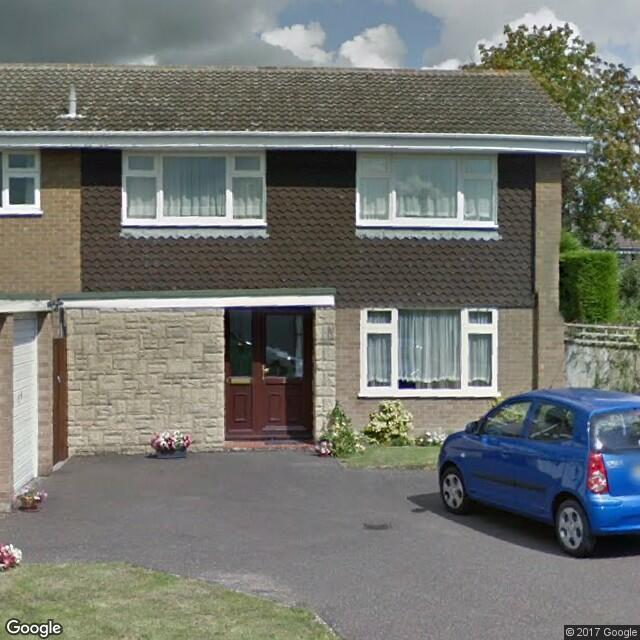
\includegraphics[width=45px]{/home/thies/db/Cambridge/data/images/cambridge/0001000009992776_QxMV8eRavS1riXfGzpSkBw.jpg} & 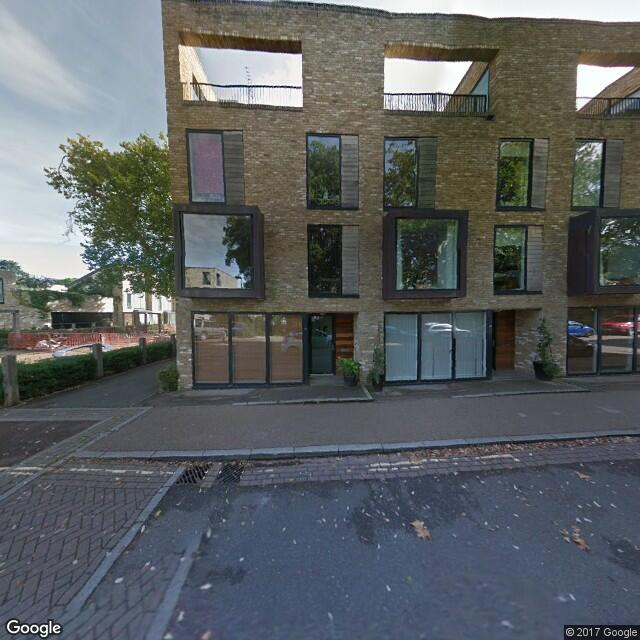
\includegraphics[width=45px]{/home/thies/db/Cambridge/data/images/cambridge/1000002500555341_NVXmLF7mim1nGBZAdgw_ew.jpg} & 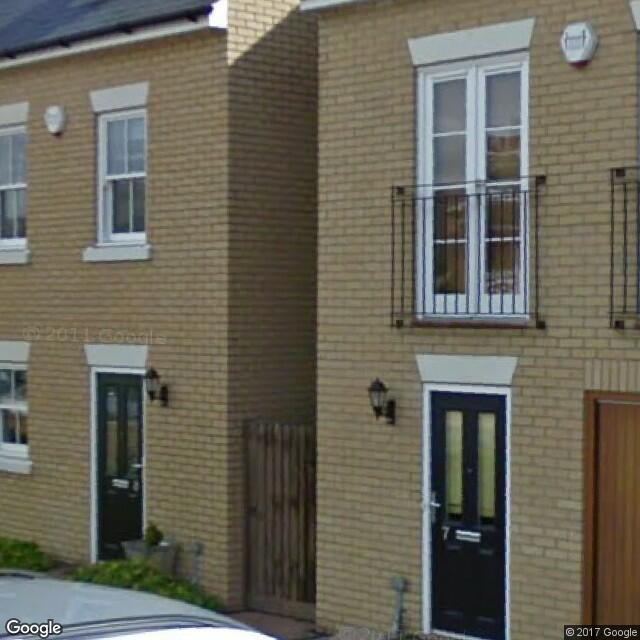
\includegraphics[width=45px]{/home/thies/db/Cambridge/data/images/cambridge/1000002500569086_g5RwBQ7D5edS2obfSogNIw.jpg} \\ 
  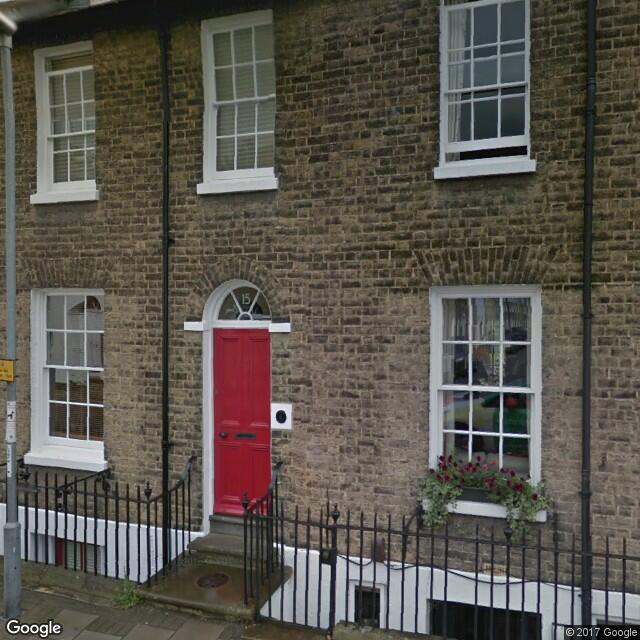
\includegraphics[width=45px]{/home/thies/db/Cambridge/data/images/cambridge/0001000010060139_8_DVq9QCmlMezNuDHGixwg.jpg} & 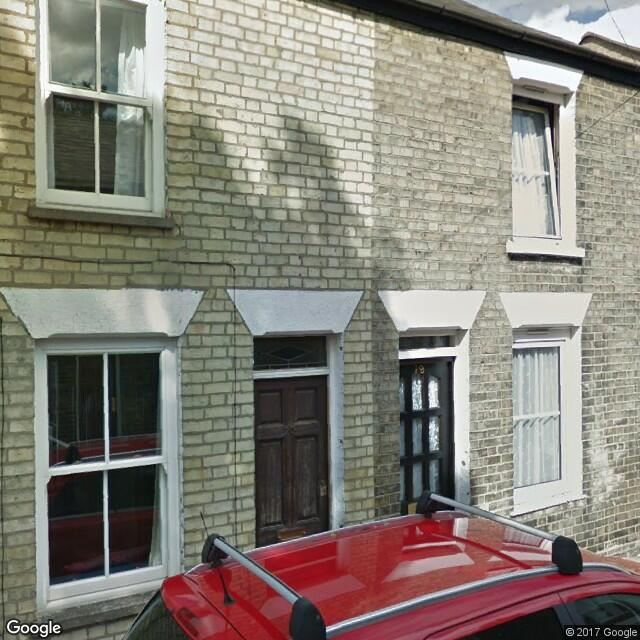
\includegraphics[width=45px]{/home/thies/db/Cambridge/data/images/cambridge/0001000010101711_wNQ403N-0pQd5fChNztfYA.jpg} & 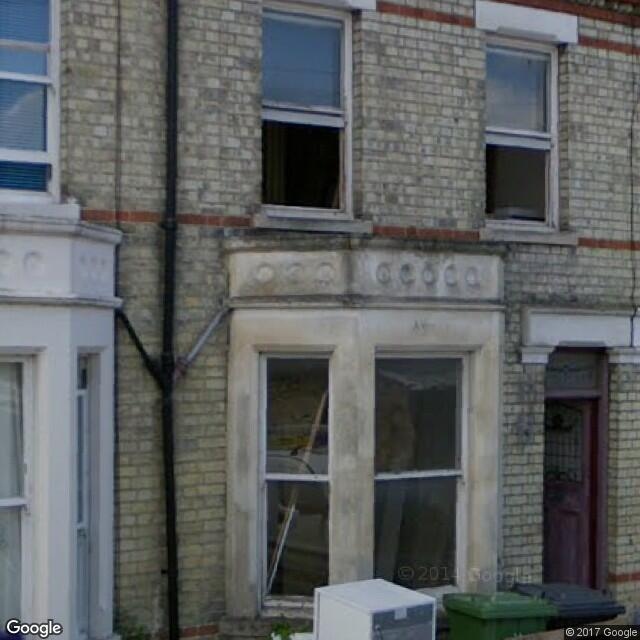
\includegraphics[width=45px]{/home/thies/db/Cambridge/data/images/cambridge/0001000010021374_55tKverBLF4C0oo8U4XABg.jpg} & 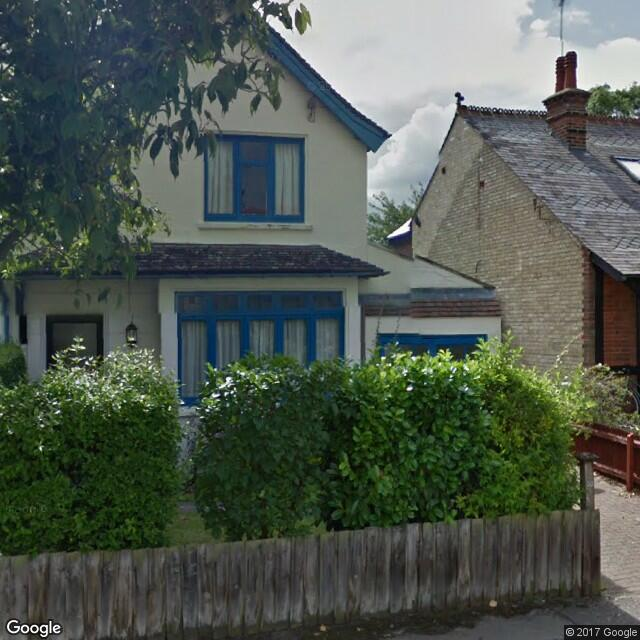
\includegraphics[width=45px]{/home/thies/db/Cambridge/data/images/cambridge/0001000010065352_kDKqKaGpPwLeCBKJIQmeCg.jpg} & 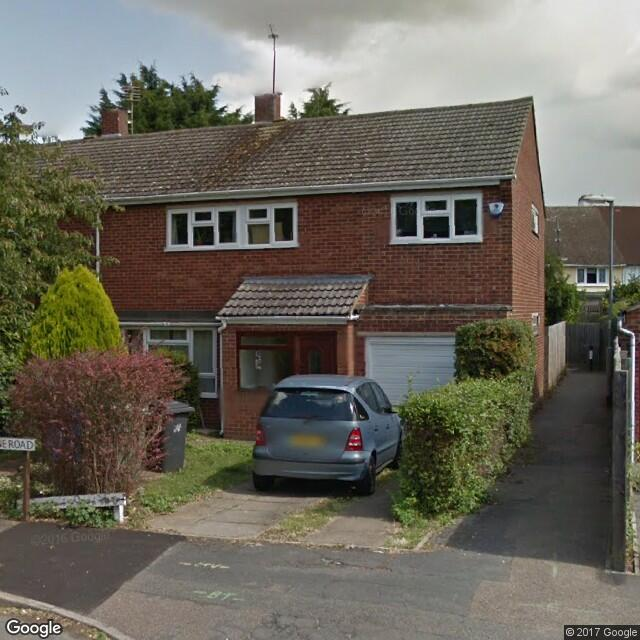
\includegraphics[width=45px]{/home/thies/db/Cambridge/data/images/cambridge/0001000010015484_zlR1vVJ7F0L6hcsFoZEydw.jpg} & 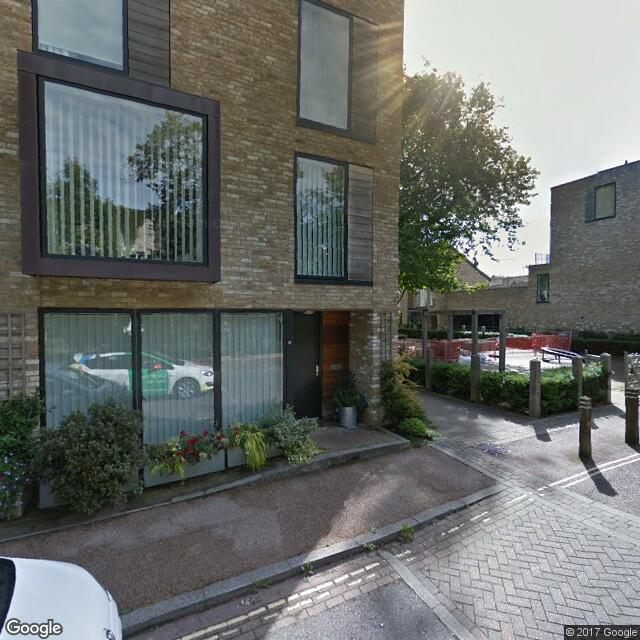
\includegraphics[width=45px]{/home/thies/db/Cambridge/data/images/cambridge/1000002500548748_i6QAKtN2HhGsTVDBan2DKw.jpg} & 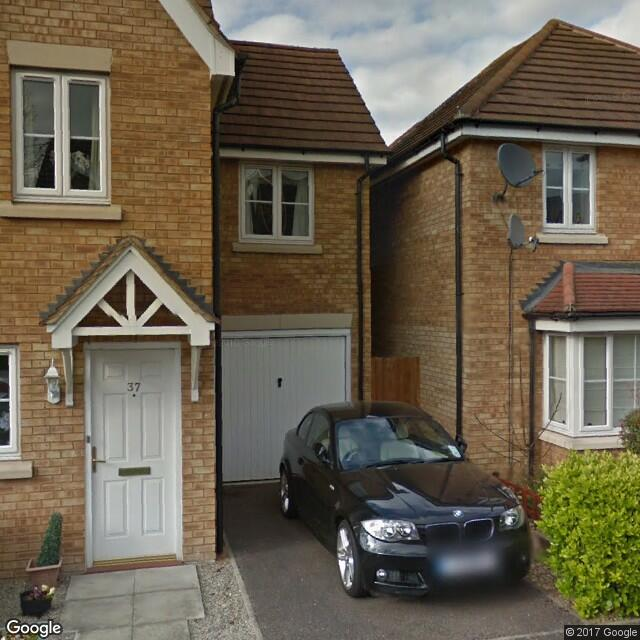
\includegraphics[width=45px]{/home/thies/db/Cambridge/data/images/cambridge/1000002057955271_dMXMWNaIwddWdHidEuXowA.jpg} \\ 
  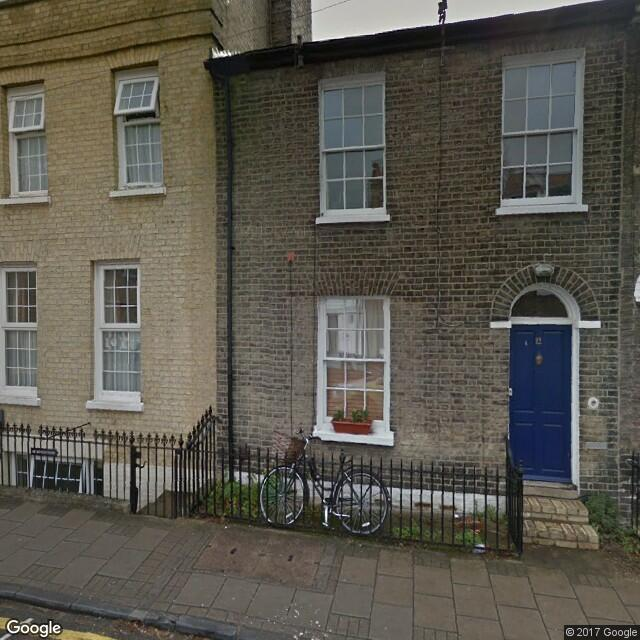
\includegraphics[width=45px]{/home/thies/db/Cambridge/data/images/cambridge/0001000010060141_W3ZIE8mPY6LJb-_hKatlUw.jpg} & 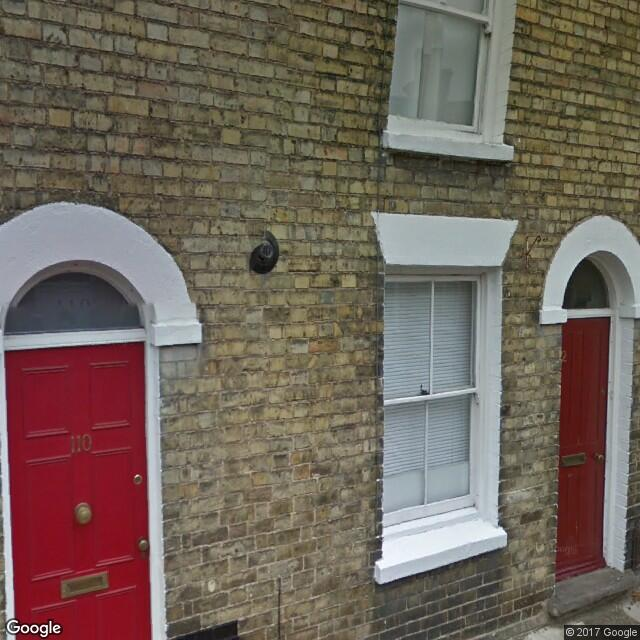
\includegraphics[width=45px]{/home/thies/db/Cambridge/data/images/cambridge/0001000010103226_XO6qx_5Q9tNnNF958OBO3g.jpg} & 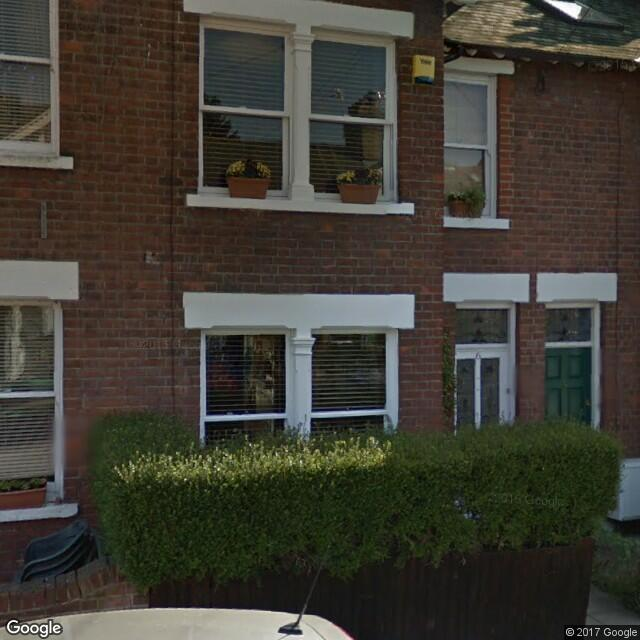
\includegraphics[width=45px]{/home/thies/db/Cambridge/data/images/cambridge/0001000010017109_MbGvl1GxhZjQ_qhD7puDBw.jpg} & 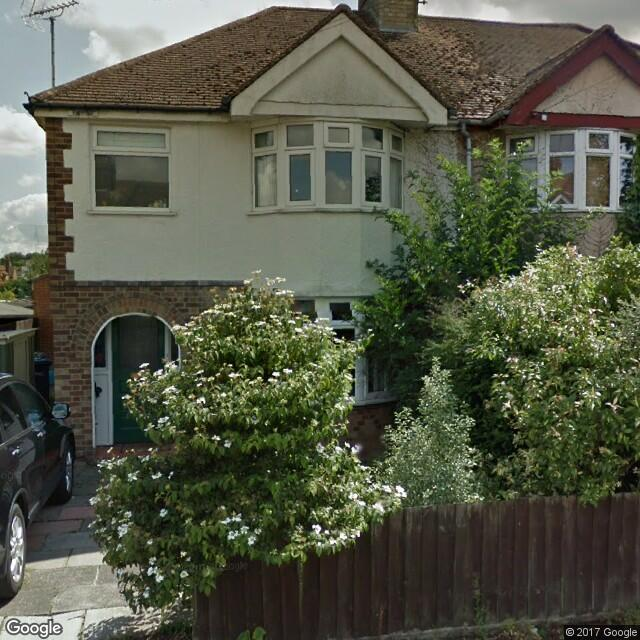
\includegraphics[width=45px]{/home/thies/db/Cambridge/data/images/cambridge/0001000009995496_N4NgCofyWASyYfcSPTjdBA.jpg} & 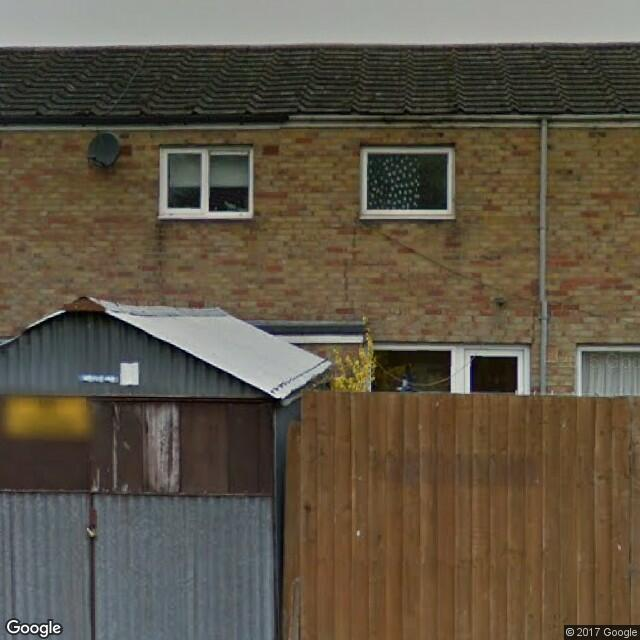
\includegraphics[width=45px]{/home/thies/db/Cambridge/data/images/cambridge/0001000010068890_aswyTpwrE_IfdbINnYx7XQ.jpg} & 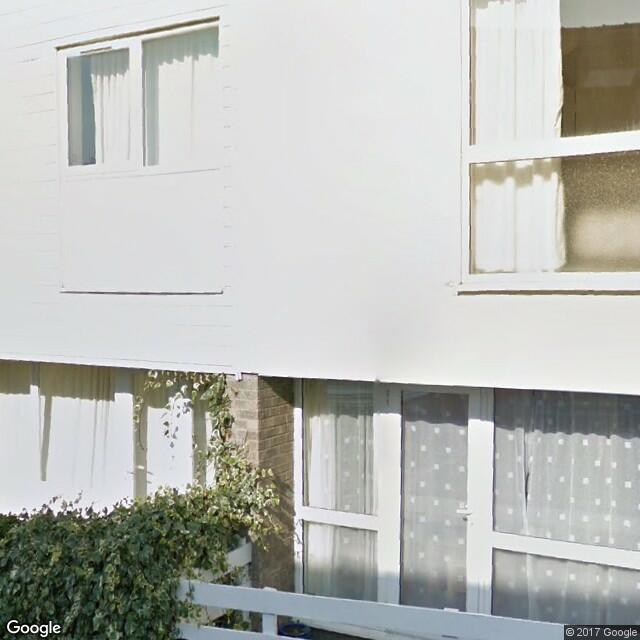
\includegraphics[width=45px]{/home/thies/db/Cambridge/data/images/cambridge/0001000010104229_qFV1-weLxn8SRW4Ib2wexQ.jpg} & \includegraphics[width=45px]{/home/thies/db/Cambridge/data/images/cambridge/0001000010199676_smIagQ34MLIcJOrjvIu9uw.jpg} \\ 
  \includegraphics[width=45px]{/home/thies/db/Cambridge/data/images/cambridge/0001000010059966_e8c8bmHUpyKpiIZ1YO9ypg.jpg} & \includegraphics[width=45px]{/home/thies/db/Cambridge/data/images/cambridge/0001000010101704_ZQFxujswdAj7EGqRlp8sXQ.jpg} & \includegraphics[width=45px]{/home/thies/db/Cambridge/data/images/cambridge/0001000010017361_WxMCM3nht5EX_K9pqIK-kQ.jpg} & \includegraphics[width=45px]{/home/thies/db/Cambridge/data/images/cambridge/0001000010066620_4TqmJVLf3urSJo4ESg1zfw.jpg} & \includegraphics[width=45px]{/home/thies/db/Cambridge/data/images/cambridge/0001000010023689_KpXUKEdjoQ9swgoB2oXA3w.jpg} & \includegraphics[width=45px]{/home/thies/db/Cambridge/data/images/cambridge/1000002500748058_DkW5iwQYtGox02-tF2i9rQ.jpg} & \includegraphics[width=45px]{/home/thies/db/Cambridge/data/images/cambridge/0001000010066718_dJmIRHcgebzrGzDR_Cahaw.jpg} \\ 
  \includegraphics[width=45px]{/home/thies/db/Cambridge/data/images/cambridge/0001000010060813_VlKeIvrTv6UwOE9HD2LgJg.jpg} & \includegraphics[width=45px]{/home/thies/db/Cambridge/data/images/cambridge/0001000010103859_P5YwPMree6QCxExkKqIzbw.jpg} & \includegraphics[width=45px]{/home/thies/db/Cambridge/data/images/cambridge/0001000010141515_5g5Bhsn_4iW-90aFMrIaSA.jpg} & \includegraphics[width=45px]{/home/thies/db/Cambridge/data/images/cambridge/0001000010066361_gliMrVbagcfkfZjLw4mKlw.jpg} & \includegraphics[width=45px]{/home/thies/db/Cambridge/data/images/cambridge/1000002500527045_p4zTtg8OzsbWjHYscCf-rA.jpg} & \includegraphics[width=45px]{/home/thies/db/Cambridge/data/images/cambridge/1000002500748076_zDr74LLmVeyKyx7dPnXK6A.jpg} & \includegraphics[width=45px]{/home/thies/db/Cambridge/data/images/cambridge/1000002500413682_drSMg0SQ9TU4Og8pXOgSxw.jpg} \\ 
  \includegraphics[width=45px]{/home/thies/db/Cambridge/data/images/cambridge/0001000010059967_e8c8bmHUpyKpiIZ1YO9ypg.jpg} & \includegraphics[width=45px]{/home/thies/db/Cambridge/data/images/cambridge/0001000010103388_CZH157SXYmF3dEVMKlWBfQ.jpg} & \includegraphics[width=45px]{/home/thies/db/Cambridge/data/images/cambridge/0001000010025644_bJ8zv37pDsP0CImvDMKC0w.jpg} & \includegraphics[width=45px]{/home/thies/db/Cambridge/data/images/cambridge/0001000010144910_COpJNwPw67J78VXCoN_HMA.jpg} & \includegraphics[width=45px]{/home/thies/db/Cambridge/data/images/cambridge/0001000009992797_JUTa4GsWaXplyCP6XeVAvw.jpg} & \includegraphics[width=45px]{/home/thies/db/Cambridge/data/images/cambridge/1000002500086356_n92s3snPX2zAwEiJnA-Pxg.jpg} & \includegraphics[width=45px]{/home/thies/db/Cambridge/data/images/cambridge/0001000010176201_dDyXoyEbeMXUhCagwazbiA.jpg} \\ 
   \hline
\end{tabular}
\label{fig:vint_examples}
\begin{minipage}{0.7\textwidth}
\footnotesize \emph{Notes:} For a brief discussion of the building styles see page \pageref{def_eras}.
\end{minipage}
\end{figure}

\begin{figure}[htb!]
  \caption{Difference of $F_1$-scores: spatial model vs. base model }
  \centering
    \includegraphics[width=0.8\textwidth]{figures/barplot_f1scores.jpg}
  \label{fig:boxplot}
\begin{minipage}{0.7\textwidth}
\vspace{0.25cm}
\footnotesize \emph{Notes:} The bar plot shows difference in the $F_1$-scores per category for the classifiers using both building level and neighbor information (dark and light blue) vs. a classifier using building level information only (red).
\end{minipage}
\end{figure}

\begin{table}[htb!]
\caption{Machine style classifications as dependent variables (Eq. \ref{eq:rev} AIC comparison) }
\label{tab:aic}
\centering
\begin{tabular}{lrrrr}
  \toprule
 & \emph{No ML pred.} & \emph{Base pred.} & \emph{Spatial pred., all} & \emph{Spatial pred., high certainty} \\ 
  \midrule
  Georgian & 1,282 & 1,052 & 1,037 & 714 \\ 
  Early Victorian & 10,231 & 7,597 & 7,259 & 4,594 \\ 
  Late Vic./Edw. & 16,204 & 11,059 & 10,491 & 6,173 \\ 
  Interwar & 18,333 & 14,471 & 13,637 & 7,670 \\ 
  Postwar & 16,845 & 14,873 & 14,648 & 7,613 \\ 
  Contemporary & 2,885 & 2,281 & 2,240 & 1,054 \\ 
  Revival & 3,336 & 2,564 & 2,480 & 1,089 \\ 
   \bottomrule
\end{tabular}
\begin{minipage}{0.7\textwidth}
\vspace{0.25cm}
\footnotesize \emph{Notes:}
AIC values for 28 binomial models in which the occurrence of building styles (in rows) is explained by hedonic characteristics, location and time dummies (Column 1), augmented by the base ML predictor (Column 2), the suggested spatial ML predictor (Column 3 \& 4). Across building styles, the AIC are lowest for the spatial ML predictor, especially when uncertain predictions are omitted (Column 4). This suggests that the spatial predictor performs best.
\end{minipage}
\end{table}

\begin{table}[!htbp] \centering 
  \caption{Hedonic Regression Estimates} 
  \label{tab:hedreg} 
\footnotesize 
\begin{tabular}{@{\extracolsep{5pt}}lcccccccc} 
\toprule
 & \multicolumn{6}{c}{Dependent variable: \emph{ln(price)}} \\ 
\cmidrule{2-9} 
 & (1) & (2) & (3) & (4) & (5) & (6) & (7) & (8)\\ 
\midrule
Constant & 13.20$^{***}$ & 13.45$^{***}$ & 13.29$^{***}$ & 13.21$^{***}$ & 15.61$^{***}$ & 18.89$^{***}$ & 13.14$^{***}$ & 13.20$^{***}$ \\ 
  & (0.20) & (0.17) & (0.20) & (1.74) & (1.72) & (3.77) & (0.20) & (0.20) \\ 
  ln(dist. city center) & $-$0.45$^{***}$ & $-$0.50$^{***}$ & $-$0.47$^{***}$ & $-$0.48$^{**}$ & $-$0.72$^{***}$ & $-$1.12$^{***}$ & $-$0.44$^{***}$ & $-$0.45$^{***}$ \\ 
  & (0.03) & (0.02) & (0.03) & (0.23) & (0.21) & (0.07) & (0.03) & (0.03) \\ 
  Type: semi-detached & $-$0.12$^{***}$ & $-$0.14$^{***}$ & $-$0.13$^{***}$ & 0.01 & $-$0.12$^{**}$ & $-$0.10 & $-$0.13$^{***}$ & $-$0.13$^{***}$ \\ 
  & (0.01) & (0.01) & (0.01) & (0.04) & (0.05) & (0.07) & (0.01) & (0.01) \\ 
  Type: terraced & $-$0.19$^{***}$ & $-$0.20$^{***}$ & $-$0.19$^{***}$ & $-$0.01 & $-$0.10$^{*}$ & $-$0.12 & $-$0.20$^{***}$ & $-$0.20$^{***}$ \\ 
  & (0.01) & (0.01) & (0.01) & (0.04) & (0.05) & (0.11) & (0.01) & (0.01) \\ 
  ln(area) & 0.40$^{***}$ & 0.40$^{***}$ & 0.40$^{***}$ & 0.33$^{***}$ & 0.29$^{***}$ & 0.21$^{***}$ & 0.39$^{***}$ & 0.39$^{***}$ \\ 
  & (0.01) & (0.01) & (0.01) & (0.07) & (0.09) & (0.01) & (0.01) & (0.01) \\ 
  ln(volume) & 0.01$^{***}$ & 0.01$^{***}$ & 0.01$^{***}$ & 0.01 & 0.02$^{***}$ & 0.02 & 0.01$^{***}$ & 0.01$^{***}$ \\ 
  & (0.001) & (0.001) & (0.001) & (0.01) & (0.01) & (0.09) & (0.001) & (0.002) \\ 
  New & 0.09$^{***}$ & 0.18$^{***}$ & 0.13$^{***}$ &  &  &  & 0.11$^{***}$ & 0.10$^{***}$ \\ 
  & (0.02) & (0.01) & (0.02) &  &  &  & (0.02) & (0.02) \\ 
  \cmidrule{2-9}
  & \multicolumn{8}{c}{\emph{Base: Contemporary}} \\
  Georgian & $-$0.04 & 0.06$^{***}$ & $-$0.04 &  &  &  & 0.01 & 0.15$^{**}$ \\ 
  & (0.03) & (0.02) & (0.03) &  &  &  & (0.03) & (0.06) \\ 
  Early Vic. & $-$0.13$^{***}$ & $-$0.01 & $-$0.11$^{***}$ &  &  &  & $-$0.04$^{**}$ & 0.01 \\ 
  & (0.02) & (0.01) & (0.02) &  &  &  & (0.02) & (0.07) \\ 
  Late Vic./Edw. & 0.01 & 0.11$^{***}$ & 0.04$^{**}$ &  &  &  & 0.06$^{***}$ & 0.15$^{**}$ \\ 
  & (0.02) & (0.01) & (0.02) &  &  &  & (0.02) & (0.08) \\ 
  Interwar & $-$0.15$^{***}$ & $-$0.02$^{**}$ & $-$0.13$^{***}$ &  &  &  & $-$0.08$^{***}$ & $-$0.15$^{**}$ \\ 
  & (0.02) & (0.01) & (0.02) &  &  &  & (0.02) & (0.06) \\ 
  Postwar & $-$0.22$^{***}$ & $-$0.06$^{***}$ & $-$0.19$^{***}$ &  &  &  & $-$0.12$^{***}$ & $-$0.17$^{***}$ \\ 
  & (0.02) & (0.01) & (0.02) &  &  &  & (0.02) & (0.04) \\ 
  Revival & 0.04$^{**}$ & 0.05$^{***}$ & 0.03 & $-$0.10 & 0.13$^{***}$ & 0.12 & 0.05$^{**}$ & 0.07$^{*}$ \\ 
  & (0.02) & (0.01) & (0.02) & (0.09) & (0.04) &  (0.09) & (0.02) & (0.04) \\ 
    \cmidrule{2-9}
  & \multicolumn{8}{c}{\emph{Base: Neigh. Contemporary}} \\

   Neigh: Georgian &  &  &  &  &  &  & $-$0.10$^{**}$ & $-$0.44$^{***}$ \\ 
  &  &  &  &  &  &  & (0.04) & (0.05) \\ 
  Neigh: Early Vic. &  &  &  &  &  &  & $-$0.13$^{***}$ & $-$0.15$^{***}$ \\ 
  &  &  &  &  &  &  & (0.02) & (0.04) \\ 
  Neigh: Late V./Edw. &  &  &  &  &  &  & $-$0.05$^{**}$ & $-$0.15$^{*}$ \\ 
  &  &  &  &  &  &  & (0.02) & (0.08) \\ 
  Neigh: Interwar &  &  &  &  &  &  & $-$0.11$^{***}$ & $-$0.01 \\ 
  &  &  &  &  &  &  & (0.02) & (0.04) \\ 
  Neigh: Postwar &  &  &  &  &  &  & $-$0.14$^{***}$ & $-$0.24$^{***}$ \\ 
  &  &  &  &  &  &  & (0.02) & (0.04) \\ 
  Neigh: Revival &  &  &  &  &  &  & $-$0.03 & $-$0.03 \\ 
  &  &  &  &  &  &  & (0.02) & (0.06) \\  
\midrule
Year dummies & Yes & Yes & Yes & Yes & Yes & Yes & Yes & Yes \\ 
Neigh. dummies & Yes & Yes & Yes & Yes & Yes & Yes & Yes & Yes \\ 
Interaction terms & No & No & No & No & No & No & No & Table \ref{tab:hedregint} \\ 
Observations & 15,642 & 23,415 & 15,721 & 377 & 567 & 348 & 15,503 & 15,503 \\ 
Adjusted R$^{2}$ & 0.88 & 0.88 & 0.88 & 0.93 & 0.91 & 0.92 & 0.89 & 0.89 \\ 
\bottomrule
\end{tabular} 
\begin{minipage}{\textwidth}
\vspace{0.25cm}
\footnotesize \emph{Notes:} $^{*}$p$<$0.1; $^{**}$p$<$0.05; $^{***}$p$<$0.01. Standard errors are robust (White's estimator). Models (1) and (4) are estimated using the architects' classifications only. Models (2) and (5) are estimated based on all observations that have been automatically classified. Models (3) and (6) are also based on automatic classifications but the sample is reduced to high confidence predictions only. Models (4-6) are estimated on sales of newly completed buildings only. The interaction terms for Model (8) are in Table \ref{tab:hedregint}.  
\end{minipage}
\end{table}

\begin{table}[ht]
\caption{Counts: Building style and neighboring buildings' style}
\label{tab:vintneigh}
\centering
\begin{tabular}{lrrrrrrr}
\toprule
\emph{Neigh.} & \multicolumn{7}{c}{\emph{Building}} \\
 \cmidrule(lr){1-1}
 \cmidrule(lr){2-8}
& \emph{Georg.} & \emph{Early Vic.} & \emph{Late V./Edw.} & \emph{Interw.} & \emph{Postw.} & \emph{Cont.} & \emph{Revival} \\ 
  \cmidrule(lr){2-8}
Georgian & 164 &  44 &   7 &   0 &   0 &   0 &   1 \\ 
  Early Vic. &  20 & 2205 & 274 &  34 &  18 &  18 &  27 \\ 
  Late Vic./Edw. &  22 & 473 & 3128 & 226 &  22 &   9 &  10 \\ 
  Interwar &   7 &  47 & 176 & 4165 & 450 &  22 &  45 \\ 
  Postwar &   1 &  10 &  25 & 553 & 2712 &  38 &  32 \\ 
  Contemporary &   0 &   0 &   5 &  16 &  42 & 348 &  12 \\ 
  Revival &   2 &  17 &   5 &  62 &  36 &  19 & 153 \\ 
   \bottomrule
\end{tabular}
\begin{minipage}{\textwidth}
\vspace{0.25cm}
\footnotesize \emph{Notes:} The style of direct neighborhoods is defined as the most frequent detected style on the same street, within 100m. 
\end{minipage}
\end{table}

\begin{table}[ht]
\centering
\caption{Coefficients interaction terms: Building and neighborhood style}
\label{tab:hedregint}
\begin{tabular}{lccccccc}
\toprule
\emph{Neigh.} & \multicolumn{7}{c}{\emph{Building}} \\
 \cmidrule(lr){1-1}
 \cmidrule(lr){2-8}
& \emph{Georg.} & \emph{Early Vic.} & \emph{Late V./Edw.} & \emph{Interw.} & \emph{Postw.} & \emph{Cont.} & \emph{Revival} \\ 
  \cmidrule(lr){2-8}

Georgian & 0.19 & 0.25 & 0.56** & -- & -- & -- & -- \\ 
   & (0.29) & (0.25) & (0.27) & -- & -- & -- & -- \\ 
Early Vic. & -0.14 & -0.04 & -0.13 & 0.03 & 0.07 & -- & 0.10 \\ 
  & (0.18) & (0.09) & (0.12) & (0.09) & (0.08) & -- & (0.10) \\ 
Late V./Edw. & -0.004 & 0.002 & -0.01 & 0.18* & 0.08 & -- & 0.13 \\ 
   & (0.19) & (0.11) & (0.13) & (0.10) & (0.10) & -- & (0.12) \\ 
Interwar & -0.23 & -0.20** & -0.17 & -0.03 & -0.07 & -- & -0.15 \\ 
  & (0.19) & (0.09) & (0.11) & (0.08) & (0.06) & -- & (0.09) \\ 
Postwar & 0.18 & 0.03 & -0.05 & 0.15** & 0.14*** & -- & 0.01 \\ 
   & (0.28) & (0.11) & (0.12) & (0.07) & (0.05) & -- & (0.09) \\ 
Contemporary & -- & -- & -- & -- & -- & -- & -- \\ 
  & -- & -- & -- & -- & -- & -- & -- \\ 
  Revival & -- & -- & -0.43*** & 0.09 & 0.04 & -- & -0.04 \\ 
   & -- & -- & (0.15) & (0.08) & (0.07) & -- & (0.09) \\ 
\bottomrule
\end{tabular}
\begin{minipage}{\textwidth}
\vspace{0.25cm}
\footnotesize \emph{Notes:} $^{*}$p$<$0.1; $^{**}$p$<$0.05; $^{***}$p$<$0.01. Standard errors are robust (White's estimator). This table features the coefficients for interaction terms of building style and neighborhood styles only, while Table \ref{tab:hedreg}, Column 8 presents all other coefficients for this model.
\end{minipage}

\end{table}

\begin{table}[ht]
\centering
\caption{Combined effect: Sum of direct, neighborhood and interaction coefficients}
\label{tab:comb}
\begin{tabular}{lccccccc}
\toprule
\emph{Neigh.} & \multicolumn{7}{c}{\emph{Building}} \\
 \cmidrule(lr){1-1}
 \cmidrule(lr){2-8}
& \emph{Georg.} & \emph{Early Vic.} & \emph{Late V./Edw.} & \emph{Interw.} & \emph{Postw.} & \emph{Cont.} & \emph{Revival} \\ 
  \cmidrule(lr){2-8}
Georgian & -0.11 & -0.17 & 0.27 & -- &--  & -0.44 &--  \\ 
  Early Vic. & -0.15 & -0.18 & -0.13 & -0.28 & -0.25 & -0.15 & 0.02 \\ 
  Late Vic./Edw. & -0.00 & -0.13 & -0.00 & -0.12 & -0.24 & -0.15 & 0.06 \\ 
  Interwar & -0.10 & -0.19 & -0.03 & -0.20 & -0.26 & -0.01 & -0.09 \\ 
  Postwar & 0.09 & -0.19 & -0.13 & -0.23 & -0.27 & -0.24 & -0.16 \\ 
  Contemporary & 0.15 & 0.01 & 0.15 & -0.15 & -0.17 & 0.00 & 0.07 \\ 
  Revival & -- & -- & -0.30 & -0.09 & -0.16 & -0.03 & 0.00 \\ 
\bottomrule
\end{tabular}
\begin{minipage}{\textwidth}
\vspace{0.25cm}
\footnotesize \emph{Notes:} The combined effect of building styles on property values is calculated by adding up the direct, neighborhood and interaction effects (Table \ref{tab:hedregint}). A revival building surrounded by other revival buildings, for instance, commands no premium over a contemporary building in a new neighborhood.
\end{minipage}
\end{table}

\clearpage

\hypertarget{bibliography}{%
\section*{Bibliography}\label{bibliography}}
\addcontentsline{toc}{section}{Bibliography}

\hypertarget{refs}{}
\leavevmode\hypertarget{ref-Ahlfeldt2012}{}%
Ahlfeldt, Gabriel, and Alexandra Mastro. 2012. ``Valuing Iconic Design:
Frank Lloyd Wright Architecture in Oak Park, Illinois.'' \emph{Housing
Studies} 27 (8): 1079--99.
\url{https://doi.org/10.1080/02673037.2012.728575}.

\leavevmode\hypertarget{ref-Asabere1989}{}%
Asabere, Paul K., George Hachey, and Steven Grubaugh. 1989.
``Architecture , Historic Zoning , and the Value of Homes.''
\emph{Journal of Real Estate Finance and Economics} 2 (3): 181--95.
\url{https://doi.org/10.1007/BF00152347}.

\leavevmode\hypertarget{ref-Buitelaar2017}{}%
Buitelaar, Edwin, and Frans Schilder. 2017. ``The Economics of Style:
Measuring the Price Effect of Neo-Traditional Architecture in Housing.''
\emph{Real Estate Economics} 45 (1): 7--27.
\url{https://doi.org/10.1111/1540-6229.12137}.

\leavevmode\hypertarget{ref-Coulson2008}{}%
Coulson, N. Edward, and Daniel P. McMillen. 2008. ``Estimating time, age
and vintage effects in housing prices.'' \emph{Journal of Housing
Economics} 17 (2): 138--51.
\url{https://doi.org/10.1016/j.jhe.2008.03.002}.

\leavevmode\hypertarget{ref-Nadai2016}{}%
De Nadai, Marco, Radu L. Vieriu, Gloria Zen, Stefan Dragicevic, Nikhil
Naik, Michele Caraviello, Cesar A. Hidalgo, Nicu Sebe, and Bruno Lepri.
2016. ``Are Safer Looking Neighborhoods More Lively? A Multimodal
Investigation into Urban Life,'' August.
\url{http://arxiv.org/abs/1608.00462}.

\leavevmode\hypertarget{ref-EnvironmentAgency2015}{}%
Environment Agency. 2015. ``LIDAR Composite DSM - 1m.''
\url{https://data.gov.uk/dataset/lidar-composite-dsm-1m1}.

\leavevmode\hypertarget{ref-Francke2017a}{}%
Francke, Marc K., and Alex M. van de Minne. 2017. ``Land, Structure and
Depreciation.'' \emph{Real Estate Economics} 45 (2): 415--51.
\url{https://doi.org/10.1111/1540-6229.12146}.

\leavevmode\hypertarget{ref-Fuerst2011}{}%
Fuerst, Franz, Patrick McAllister, and Claudia B Murray. 2011.
``Designer buildings: estimating the economic value of `signature'
architecture.'' \emph{Environment and Planning A} 43 (1): 166--84.
\url{https://doi.org/10.1068/a43270}.

\leavevmode\hypertarget{ref-Gebru2017}{}%
Gebru, Timnit, Jonathan Krause, Yilun Wang, Duyun Chen, Jia Deng, Erez
Lieberman Aiden, and Li Fei-Fei. 2017. ``Using Deep Learning and Google
Street View to Estimate the Demographic Makeup of the US.'' \emph{PNAS}
114 (50): 13108--13. \url{https://doi.org/10.1073/pnas.1700035114}.

\leavevmode\hypertarget{ref-Ghimire2010a}{}%
Ghimire, B., J. Rogan, and J. Miller. 2010. ``Contextual land-cover
classification: Incorporating spatial dependence in land-cover
classification models using random forests and the Getis statistic.''
\emph{Remote Sensing Letters} 1 (1): 45--54.
\url{https://doi.org/10.1080/01431160903252327}.

\leavevmode\hypertarget{ref-GlaeserKincaidNaik2018}{}%
Glaeser, Edward L., Michael Scott Kincaid, and Nikhil Naik. 2018.
``Computer Vision and Real Estate: Do Looks Matter and Do Incentives
Determine Looks?'' \url{http://www.nber.org/papers/w25174}.

\leavevmode\hypertarget{ref-Glaeser2016}{}%
Glaeser, Edward L., Scott Duke Kominers, Michael Luca, and Nikhil Naik.
2018. ``Big Data and Big Cities: The Promises and Limitations of
Improved Measures of Urban Life.'' \emph{Economic Inquiry} 56 (1):
114--37. \url{https://doi.org/10.1111/ecin.12364}.

\leavevmode\hypertarget{ref-He2016}{}%
He, Kaiming, Xiangyu Zhang, Shaoqing Ren, and Jian Sun. 2016. ``Deep
Residual Learning for Image Recognition.'' \emph{The IEEE Conference on
Computer Vision and Pattern Recognition (CVPR)}, 770--78.

\leavevmode\hypertarget{ref-Helbich2013}{}%
Helbich, Marco, Andreas Jochem, Werner Mücke, and Bernhard Höfle. 2013.
``Boosting the predictive accuracy of urban hedonic house price models
through airborne laser scanning.'' \emph{Computers, Environment and
Urban Systems} 39. Elsevier Ltd: 81--92.
\url{https://doi.org/10.1016/j.compenvurbsys.2013.01.001}.

\leavevmode\hypertarget{ref-princecharles2014}{}%
HRH The Prince of Wales. 2014. ``Facing up to the future: Prince Charles
on 21st century architecture.'' \emph{Architectural Review}, December.
\url{https://www.architectural-review.com/essays/viewpoints/facing-up-to-the-future-prince-charles-on-21st-century-architecture/8674119.article}.

\leavevmode\hypertarget{ref-LandRegistry2016a}{}%
Land Registry. 2017. ``Price Paid Data.''
\url{http://landregistry.data.gov.uk/app/ppd}.

\leavevmode\hypertarget{ref-Lindenthal2017b}{}%
Lindenthal, Thies. 2017a. ``Beauty in the Eye of the Home-Owner:
Aesthetic Zoning and Residential Property Values.'' \emph{Real Estate
Economics}, 1--26. \url{https://doi.org/10.1111/1540-6229.12204}.

\leavevmode\hypertarget{ref-Lindenthal2017}{}%
---------. 2017b. \emph{Estimating Supply Elasticities for Residential
Real Estate in the United Kingdom}. Comprehens. Elsevier Inc.
\url{https://doi.org/https://doi.org/10.1016/B978-0-12-409548-9.09682-2}.

\leavevmode\hypertarget{ref-Liu2017}{}%
Liu, Lun, Elisabete A. Silva, Chunyang Wu, and Hui Wang. 2017. ``A
machine learning-based method for the large-scale evaluation of the
qualities of the urban environment.'' \emph{Computers, Environment and
Urban Systems} 65. The Authors: 113--25.
\url{https://doi.org/10.1016/j.compenvurbsys.2017.06.003}.

\leavevmode\hypertarget{ref-Moorhouse1994}{}%
Moorhouse, John C., and Margaret Supplee Smith. 1994. ``The Market for
Residential Architecture: 19th century Row Houses in Boston's South
End.'' \emph{Journal of Urban Economics} 35 (3): 267--77.
\url{https://doi.org/10.1006/juec.1994.1016}.

\leavevmode\hypertarget{ref-Naik2017}{}%
Naik, Nikhil, Scott Duke Kominers, Ramesh Raskar, Edward L. Glaeser, and
César A. Hidalgo. 2017. ``Computer vision uncovers predictors of
physical urban change.'' \emph{Proceedings of the National Academy of
Sciences} 114 (29): 7571--6.
\url{https://doi.org/10.1073/pnas.1619003114}.

\leavevmode\hypertarget{ref-Naik2016AER}{}%
Naik, Nikhil, Ramesh Raskar, and César A. Hidalgo. 2016. ``Cities Are
Physical Too: Using Computer Vision to Measure the Quality and Impact of
Urban Appearance.'' \emph{American Economic Review} 106 (5): 128--32.
\url{https://doi.org/10.1257/aer.p20161030}.

\leavevmode\hypertarget{ref-ONS2017b}{}%
Office for National Statistics. 2017. ``A Beginner's Guide to UK
Geography.''

\leavevmode\hypertarget{ref-ONS2017}{}%
---------. 2019. ``Open Geography Portal -- 2011 Census Boundaries.''
\url{https://www.ons.gov.uk/methodology/geography/ukgeographies/censusgeography}.

\leavevmode\hypertarget{ref-OrdnanceSurvey2017}{}%
Ordnance Survey. 2017a. ``AddressBase.''
\url{https://www.ordnancesurvey.co.uk/business-and-government/help-and-support/products/addressbase-premium.html}.

\leavevmode\hypertarget{ref-OrdnanceSurvey2017a}{}%
---------. 2017b. ``OS Maps Local.''
\url{https://www.ordnancesurvey.co.uk/business-and-government/products/os-open-map-local.html}.

\leavevmode\hypertarget{ref-Plaut2006}{}%
Plaut, Steven, and Egita Uzulena. 2006. ``Architectural Design and the
Value of Housing in Riga, Latvia.'' \emph{International Real Estate
Review} 9 (1): 112--31.

\leavevmode\hypertarget{ref-Ribeiro2016}{}%
Ribeiro, Marco Tulio, Sameer Singh, and Carlos Guestrin. 2016. ``"Why
Should I Trust You?" Explaining the Predictions of Any Classifier.'' In
\emph{22nd Acm Sigkdd International Conference on Knowledge Discovery
and Data Mining}, 1135-----1144. San Francisco.

\leavevmode\hypertarget{ref-scruton2018}{}%
Scruton, Roger. 2018. ``The Fabric of the City.'' Colin Amery Memorial
Lecture. Policy Exchange.
\url{https://policyexchange.org.uk/wp-content/uploads/2018/11/The-Fabric-of-the-City.pdf}.

\leavevmode\hypertarget{ref-Szegedy2015}{}%
Szegedy, Christian, Vincent Vanhoucke, Sergey Ioffe, Jonathon Shlens,
and Zbigniew Wojna. 2015. ``Rethinking the Inception Architecture for
Computer Vision.'' \url{https://doi.org/10.1109/CVPR.2016.308}.

\leavevmode\hypertarget{ref-economistlineofbeauty2018}{}%
The Economist. 2018. ``The line of beauty.'' \emph{The Economist},
November. London.
\url{https://www.economist.com/britain/2018/11/17/how-to-defeat-nimbyism-build-more-beautiful-houses}.

\leavevmode\hypertarget{ref-Vandell1989}{}%
Vandell, Kerry D., and Jonathan S. Lane. 1989. ``The Economics of
Architecture and Urban Design: Some Preliminary Findings.'' \emph{AREUEA
Journal} 17 (2): 235--60.


\end{document}
